
\documentclass[18pt,aspectratio=169]{beamer}
%\usetheme{kit}
\usepackage{ngerman}

% metropolis theme: https://github.com/matze/mtheme
\usetheme[sectionpage=progressbar,subsectionpage=progressbar,progressbar=frametitle]{metropolis}

% Notizen
%\setbeameroption{show notes}
%\setbeameroption{show notes on second screen=right}

\setbeamertemplate{section in toc}[sections numbered]
\setbeamertemplate{subsection in toc}[subsections numbered]

%redefine note page with bigger slide
\makeatletter
\defbeamertemplate*{note page}{mynotes}
{%
	{%
		\scriptsize
		\usebeamerfont{note title}\usebeamercolor[fg]{note title}%
		\ifbeamercolorempty[bg]{note title}{}{%
			\insertvrule{.45\paperheight}{note title.bg}%
			\vskip-.45\paperheight%
			\nointerlineskip%
		}%
		\vbox{
			\hfill\insertslideintonotes{0.45}\hskip-\Gm@rmargin\hskip0pt%
			\vskip-0.45\paperheight%
			\nointerlineskip
			\begin{pgfpicture}{0cm}{0cm}{0cm}{0cm}
				\begin{pgflowlevelscope}{\pgftransformrotate{90}}
					{\pgftransformshift{\pgfpoint{-2cm}{0.2cm}}%
						\pgftext[base,left]{\usebeamerfont{note date}\usebeamercolor[fg]{note date}\the\year-\ifnum\month<10\relax0\fi\the\month-\ifnum\day<10\relax0\fi\the\day}}
				\end{pgflowlevelscope}
		\end{pgfpicture}}
		\nointerlineskip
		\vbox to .45\paperheight{\vskip0.5em
			\hbox{\insertshorttitle[width=8cm]}%
			\setbox\beamer@tempbox=\hbox{\insertsection}%
			\hbox{\ifdim\wd\beamer@tempbox>1pt{\hskip4pt\raise3pt\hbox{\vrule
						width0.4pt height7pt\vrule width 9pt
						height0.4pt}}\hskip1pt\hbox{\begin{minipage}[t]{7.5cm}\def\breakhere{}\insertsection\end{minipage}}\fi%
			}%
			\setbox\beamer@tempbox=\hbox{\insertsubsection}%
			\hbox{\ifdim\wd\beamer@tempbox>1pt{\hskip17.4pt\raise3pt\hbox{\vrule
						width0.4pt height7pt\vrule width 9pt
						height0.4pt}}\hskip1pt\hbox{\begin{minipage}[t]{7.5cm}\def\breakhere{}\insertsubsection\end{minipage}}\fi%
			}%
			\setbox\beamer@tempbox=\hbox{\insertshortframetitle}%
			\hbox{\ifdim\wd\beamer@tempbox>1pt{\hskip30.8pt\raise3pt\hbox{\vrule
						width0.4pt height7pt\vrule width 9pt
						height0.4pt}}\hskip1pt\hbox{\insertshortframetitle[width=7cm]}\fi%
			}%
			\vfil}%
	}%
	\ifbeamercolorempty[bg]{note page}{}{%
		\nointerlineskip%
		\insertvrule{.55\paperheight}{note page.bg}%
		\vskip-.55\paperheight%
	}%
	\vskip.25em
	\nointerlineskip
	\insertnote
}
\makeatother

\setbeamertemplate{note page}[mynotes]

\makeatletter
\setbeamertemplate{section page}{
	\centering
	\begin{minipage}{22em}
		\raggedright
		\usebeamercolor[fg]{section title}
		\usebeamerfont{section title}
		\thesection.~\insertsectionhead\\[-1ex]
		\usebeamertemplate*{progress bar in section page}
		\par
		\ifx\insertsubsectionhead\@empty\else%
		\usebeamercolor[fg]{subsection title}%
		\usebeamerfont{subsection title}%
		\thesection.\thesubsection~\insertsubsectionhead
		\fi
	\end{minipage}
	\par
	\vspace{\baselineskip}
}
\makeatother

\definecolor{myColor}{HTML}{4477AA}
\definecolor{pitchblack}{HTML}{000000}
\setbeamercolor{alerted text}{fg=myColor}
\setbeamercolor{frametitle}{bg=pitchblack, fg=white}

\makeatletter
\setlength{\metropolis@titleseparator@linewidth}{1pt}
\setlength{\metropolis@progressonsectionpage@linewidth}{2pt}
\setlength{\metropolis@progressinheadfoot@linewidth}{2pt}
\makeatother


% uncomment the following line if you want to hide the navigation symbols
%\beamertemplatenavigationsymbolsempty 

\title{Theoretische Informatik I}
\subtitle{Automaten und Formale Sprachen}
\author{\texorpdfstring{Peter Kossek\newline\href{mailto:e0030414@ba-sachsen.de}{\scriptsize e0030414@ba-sachsen.de}}{Peter Kossek}}

\institute{Berufsakademie Sachsen, Staatliche Studienakademie Leipzig} % Deutsch
\date{}

\makeatletter
\@addtoreset{figure}{section}
\@addtoreset{table}{section}
\makeatother

\renewcommand{\thefigure}{\thesection.\arabic{figure}}

\renewcommand{\thetable}{\thesection.\arabic{table}}

\usepackage{nameref}
\makeatletter
\newcommand*{\currentname}{\@currentlabelname}
\makeatother

\usepackage{circuitikz}
\usepackage{tikz}
\usetikzlibrary{automata, positioning, arrows}

%strikeout text in math mode
\usepackage[normalem]{ulem}
\usepackage{amsmath}
\newcommand{\stkout}[1]{\ifmmode\text{\sout{\ensuremath{#1}}}\else\sout{#1}\fi}

\usepackage{tabularx} %same-width columns
\newcolumntype{Y}{>{\centering\arraybackslash}X} %columntype Y is centered column for tabularx

\setcounter{tocdepth}{1} % only sections in TOC

\usepackage{wasysym} %for lightning symbol

\begin{document}

\selectlanguage{ngerman}
%title page
\begin{frame}
	\titlepage
\end{frame}

\begin{frame}
	\frametitle{Danksagung}
	Diese Vorlesung basiert maßgeblich auf dem Script von\\
	Prof. Dr. habil. Jochen Kripfganz\\
	Dozent für Theoretische Informatik an der BA Leipzig bis 2021
\end{frame}

\begin{frame}{Organisatorisches}
	\begin{itemize}
		\item Teil-Präsenzveranstaltung
		\item Übungen
		\item Fragen zum Lehrstoff
		\item besondere Bedürfnisse
	\end{itemize}
\end{frame}

\AtBeginSection{
	\begin{frame}
		\sectionpage
		\tableofcontents[sectionstyle=hide/hide,subsectionstyle=show/show/hide]
	\end{frame}
}

\begin{frame}
	\frametitle{Literatur}
	\begin{itemize}
		\item Script zur Vorlesung
		\begin{itemize}
			\item \url{https://github.com/bluepoke/Automaten_Formale_Sprachen}
		\end{itemize}
		\item Grundlage der Vorlesung
		\begin{itemize}
			\item Schöning, U.: \textit{Logik für Informatiker}
			\item Schöning, U.: \textit{Theoretische Informatik - kurz gefasst}
		\end{itemize}
		\item Weitere Literatur
		\begin{itemize}
			\item Vossen, G.; Witt, K. U.: \textit{Grundlagen der Theoretischen Informatik mit Anwendungen}
			\item Hollas, B.: \textit{Grundkurs Theoretische Informatik}
			\item Erk, K.;  Priese, L.: \textit{Theoretische Informatik}
		\end{itemize}
	\end{itemize}
\end{frame}

%table of contents
\begin{frame}
	\frametitle{Gliederung}
	\tableofcontents
\end{frame}

%\frame{
%	\frametitle{Sprachen im Kontext der Informatik}
%	
%	\begin{itemize}
%		\item \emph{Sprache:} Menge zulässiger Worte über einem Alphabet
%		\item \emph{Programm:} String über einem Alphabet von Eingabezeichen (Quellcode) bzw. binär über 0/1
%		\item \emph{Compiler:} 
%		\begin{itemize}
%			\item prüft die Zulässigkeit dieses Strings als Satz (Wort) einer Sprache
%			\item generiert Folge von Maschinenbefehlen
%		\end{itemize}
%		\item \emph{Lexikalische Analyse:} Übersetzer-Modul ("`Scanner"') fasst Symbolfolgen zu Schlüsselworten ("`Token"') zusammen
%		\item \emph{Syntaxanalyse:}
%		\begin{itemize}
%			\item "`Parser"' prüft, ob Folge von Token zulässig ist
%			\item Semantik-Prüfung erfolgt dabei nicht
%		\end{itemize}
%	\end{itemize}
%}

\section{Aussagenlogik}

\subsection{Aussagenlogische Formeln}

\begin{frame}{Aussagenlogik: Syntax}
	\begin{itemize}
		\item \emph{Aussage:} Satz, der entweder wahr ($w$) oder falsch ($f$) ist; Aussagenvariable $A$; Wahrheitswert $w(A)$
		\item \emph{Syntax:} Induktive Definition korrekt gebildeter aussagenlogischer Formeln F über Variablenmenge $V=\{A, B, \ldots\}$:
		\begin{itemize}
			\item Die Booleschen Wahrheitswerte $w$ und $f$ sind Formeln
			\item Jede Variable aus $V$ ist eine Formel: \emph{Atome}
			\item Negation (NICHT): $\neg F$ ist eine Formel
			\item Konjugation (UND): $(F_1 \land F_2)$ ist eine Formel
			\item Disjunktion (ODER): $(F_1 \lor F_2)$ ist eine Formel
			\item Implikation ("`wenn \ldots, dann"'): $(F_1 \rightarrow F_2)$ ist eine Formel
			\item Äquivalenz ("`genau dann, wenn"'): $(F_1 \leftrightarrow F_2)$ ist eine Formel
			\item andere Verknüpfungen bilden keine Formel
		\end{itemize}
	\end{itemize}
\end{frame}

\begin{frame}{Präzedenzregeln}
	Vereinbarung zur Reduzierung von Klammern
	\begin{itemize}
		\item Bindung (analog "`Punkt vor Strich"'-Rechnung)
		\begin{itemize}
			\item $\neg$ bindet stärker als $\land$
			\item $\land$ bindet stärker als $\lor$
			\item $\lor$ bindet stärker als $\rightarrow$ und $\leftrightarrow$
		\end{itemize}
		\item Operatoren gleicher Stärke: Auswertung linksassoziativ; z.B. \\ $(A \lor B \lor C)$ steht für $((A \lor B) \lor C)$
		\item äußere Klammer weglassen: $(((A \lor B) \rightarrow C) \land B) \mapsto (A \lor B \rightarrow C) \land B$
	\end{itemize}
\end{frame}

\begin{frame}{Semantik}
	aussagenlogischen Formeln wird eine Bedeutung zugeordnet
	\begin{itemize}
		\item Def. Belegung (Interpretation) $I: V \rightarrow \{f, w\}$\\ den Atomen wird jeweils ein konkreter Wahrheitswert zugeordnet
		\item schrittweise (über die Bewertung von Teilformeln) lassen sich dann zusammengesetzte Formeln bewertn:
		\begin{itemize}
			\item $I(\neg F)=w$ falls $I(F)=f$, sonst $I(\neg F)=f$
			\item $I(F \land G)=w$ falls $I(F)=w$ und $I(G)=w$, sonst $I(F \land G)=f$
			\item $I(F \lor G)=w$ falls $I(F)=w$ oder $I(G)=w$, sonst $I(F \lor G)=f$
			\item $I(F \rightarrow G)=w$ falls $I(F)=f$ oder $I(G)=w$, sonst $I(F \rightarrow G)=f$
			\item $I(F \leftrightarrow G)=w$ falls $I(F)=I(G)$, sonst $I(F \leftrightarrow G)=f$
		\end{itemize}
	\end{itemize}
\end{frame}

\begin{frame}{Semantik: Darstellung per Wahrheitstafel}
	Wahrheitstafel enthält zeilenweise alle möglichen Belegungen
	\begin{table}
		\centering
			\begin{tabular}{|c|c|c|c|c|c|c|}
				\hline
				$A$ & $B$ & $\neg A$ & $A \land B$ & $A \lor B$ & $A \rightarrow B$ & $A \leftrightarrow B$ \\
				\hline
				f & f & w & f & f & w & w \\
				\hline
				f & w & w & f & w & w & f \\
				\hline
				w & f & f & f & w & f & f \\
				\hline
				w & w & f & w & w & w & w \\
				\hline
			\end{tabular}
			\caption{Wahrheitstafel der Grundoperationen}
		\end{table}
		logische Äquivalenz $F_1 \equiv F_2$: $F_1$ und $F_2$ haben gleichen Wahrheitswerteverlauf; z.B.\\
		$A \rightarrow B \equiv \neg A \lor B$\\
		$A \leftrightarrow B \equiv (A \rightarrow B) \land (B \rightarrow A)$
\end{frame}

\begin{frame}{Erfüllbarkeit, Tautologie, Kontradiktion}
	\begin{itemize}
		\item Sei $F$ eine Formel und $I$ eine Belegung. Falls $I$ für alle in $F$ vorkommenden Atome definiert ist, so heißt $I$ \underline{zu $F$ passend}
		\item Falls $I$ zu $F$ passend ist, und es gilt $I(F)=w$, dann heißt $I$ \underline{Modell für $F$}; Schreibweise: $I \models F$
		\item $F$ heißt \underline{erfüllbar}, falls $F$ mindestens ein Modell besitzt; sonst heißt $F$ \underline{unerfüllbar} (Kontradiktion; Schreibweise $F\bot$)
		\item $F$ heißt gültig bzw. \underline{Tautologie}, falls jede zu $F$ passende Belegung $I$ ein Modell für $F$ ist; Schreibweise $\models F$ oder $F\top$ \\
		Beispiel: $(A \land B) \rightarrow A$
		\item es gilt: $F$ ist Tautologie gdw. $\neg F$ ist Kontradiktion
	\end{itemize}
\end{frame}

\begin{frame}{Äquivalenz aussagenlogischer Formeln}
	\begin{itemize}
		\item Zwei Formeln $F$ und $G$ heißen äquivalent ($F \equiv G$), falls für alle Belegungen $I$ gilt: $I(F)=I(G)$
		\item Äquivalenz kann bewiesen (oder widerlegt) werden durch aufstellen der jeweiligen Wahrheitstafeln
		\item Beispiele
		\begin{itemize}
			\item $A \rightarrow B \equiv \neg A \lor B$
			\item $A \leftrightarrow B \equiv (A \land B) \lor (\neg A \land \neg B) \equiv (A \rightarrow B) \land (B \rightarrow A)$
		\end{itemize}
		\item Ersetzbarkeitstheorem:\\
		enthält eine Formel $F$ eine Teilformel $G$ und wird $G$ durch eine äquivalente Formel ersetzt, so entsteht eine zu $F$ äquivalente Formel
	\end{itemize}
\end{frame}

\begin{frame}{Äquivalenzen als Rechenregeln}
	\begin{itemize}
		\item Idempotenz
		\begin{itemize}
			\item $(A \land A) \equiv A$
			\item $(A \lor A) \equiv A$
		\end{itemize}
		\item Kommutativgesetz
		\begin{itemize}
			\item $(A \land B) \equiv (B \land A)$
			\item $(A \lor B) \equiv (B \lor A)$
		\end{itemize}
		\item Assoziativgesetz
		\begin{itemize}
			\item $(A \land (B \land C)) \equiv ((A \land B) \land C)$
			\item $(A \lor (B \lor C)) \equiv ((A \lor B) \lor C)$
		\end{itemize}
		\item Distributivgesetz
		\begin{itemize}
			\item $(A \land (B \lor C)) \equiv ((A \land B) \lor (A \land C))$
			\item $(A \lor (B \land C)) \equiv ((A \lor B) \land (A \lor C))$
		\end{itemize}
	\end{itemize}
\end{frame}

\begin{frame}{Äquivalenzen als Rechenregeln (Fortsetzung)}
	\begin{itemize}
		\item Absorptionsgesetz
		\begin{itemize}
			\item $(A \land (A \lor B)) \equiv A$
			\item $(A \lor (A \land B)) \equiv A$
		\end{itemize}
		\item Doppelnegation
		\begin{itemize}
			\item $\neg \neg A \equiv A$
		\end{itemize}
		\item deMorgansche Regeln
		\begin{itemize}
			\item $\neg (A \land B) \equiv (\neg A \lor \neg B)$
			\item $\neg (A \lor B) \equiv (\neg A \land \neg B)$
		\end{itemize}
		\item Tautologieregeln: sei $A$ Tautologie; $A\top$ bzw. $\models A$
		\begin{itemize}
			\item $(A \lor B) \equiv A$; $(A \land B) \equiv B$
		\end{itemize}
		\item Kontradiktionsregeln: sei $A$ Kontradiktion; $A\bot$
		\begin{itemize}
			\item $(A \lor B) \equiv B$; $(A \land B) \equiv A$
		\end{itemize}
	\end{itemize}
\end{frame}

\begin{frame}{Beispiel: direkter Beweis der Gültigkeit einer Formel (als Alternative zur Wahrheitstafel)}
	\begin{columns}
		\column{.5\textwidth}
		\begin{eqnarray*}
				F &=& (A \land (A \rightarrow B)) \rightarrow B\\
				  &\equiv& \neg (A \land (A \rightarrow B)) \lor B\\
				  &\equiv& \neg (A \land (\neg A \lor B)) \lor B\\
				  &\equiv& \neg A \lor \neg(\neg A \lor B) \lor B\\
				  &\equiv& \neg A \lor (A \land \neg B) \lor B\\
				  &\equiv& \neg A \lor (A \lor B) \land (\neg B \lor B)\\
				  &\equiv& \neg A \lor (A \lor B) \land w\\
				  &\equiv& \neg A \lor A \lor B\\
				  &\equiv& w \lor B\\
				  &\equiv& w
		\end{eqnarray*}
		\column{.5\textwidth}
		\begin{table}
			\begin{tabular}{|c|c|c|c|c|}
				\hline
				$A$ & $B$ & $A \rightarrow B$ & $A \land (A \rightarrow B)$ & $F$ \\
				\hline
				f & f & w & f & w \\
				\hline
				f & w & w & f & w \\
				\hline
				w & f & f & f & w \\
				\hline
				w & w & w & w & w \\
				\hline
			\end{tabular}
			\caption{Wahrheitstafel}
			\label{tblWahrheitswerteGrundoperationen}
		\end{table}
	\end{columns}		
\end{frame}

\begin{frame}{Normalformen}
	\begin{itemize}
		\item \emph{Literal:} Aussagenvariable $A$ ("`positives Literal"') oder negierte Aussagenvariable $\neg A$ ("`negatives Literal"')
		\item \emph{Negationsnormalform (NNF)}: Formel $F$ ist in NNF, falls $\rightarrow$ und $\leftrightarrow$ aufgelöst sind und alle Negationszeichen $\neg$ unmittelbar vor einer Aussagenvariable stehen.\\
		beachte: NNF ist nicht eindeutig
		\item \emph{Monom:} Konjunktion von Literalen, d.h. Formel der Art\\
		$\bigwedge_iL_i=L_1\land L_2\land\ldots\land L_k$
		\item \emph{Klausel:} Disjunktion von Literalen, d.h. Formel der Art\\
		$\bigvee_iL_i=L_1\lor L_2\lor\ldots\lor L_k$
	\end{itemize}
\end{frame}

\begin{frame}{Disjunktive Normalform (DNF) und Konjunktive Normalform (KNF)}
	\begin{itemize}
		\item Disjunktive Normalform \emph{DNF:} Disjunktion von Konjunktionen (Monomen)\\
		$F=\bigvee_i\left(\bigwedge_jL_{ij}\right)$
		\item Konjunktive Normalform \emph{KNF:} Konjunktion von Disjunktionen (Klauseln)\\
		$F=\bigwedge_i\left(\bigvee_jL_{ij}\right)$
		\item Für jede Formel existiert eine äquivalente Formel in KNF und eine äquivalente Formel in DNF
		\begin{itemize}
			\item Erzeuge NNF $\mapsto$ DNF bzw. KNF\\
			DNF: ersetze Ausdrücke der Art $(F \land (G \lor H))$ durch $(F \land G) \lor (F \land H)$ solange solche Teilformen existieren\\
			KNF: ersetze Ausdrücke der Art $(F \lor (G \land H))$ durch $(F \lor G) \land (F \lor H)$ solange solche Teilformeln existieren
		\end{itemize}
	\end{itemize}
\end{frame}

\begin{frame}{Konstruktion kanonische DNF/KNF aus Wahrheitstafel}
	\begin{itemize}
		\item \emph{Kanonische} DNF bzw. KNF: jede Aussagenvariable kommt in jedem Monom bzw. jeder Klausel genau einmal vor (positiv oder negativ)
		\item Kanonische NF lassen sich aus der Wahrheitstafel der Formel ablesen
		\begin{itemize}
			\item Kanonische DNF (KDNF)
			\begin{itemize}
				\item Je ein Monom für jede Belegung mit Wahrheitswert $w$
				\item Setze $L_j=A_j$, falls $w(A_j)=w$, $L_j=\neg A_j$ sonst
			\end{itemize}
			\item Kanonische KNF (KKNF)
			\begin{itemize}
				\item Je eine Klausel für jede Belegung mit Wahrheitswert $f$
				\item Setze $L_j=\neg A_j$, falls $w(A_j)=w$, $L_j=A_j$ sonst
			\end{itemize}
		\end{itemize}
		\item Übungsbeispiel (KNF, aber nicht kanonisch)\\
		$F=\neg B \land (A \lor \neg C)$
	\end{itemize}
\end{frame}

\begin{frame}{Beispiel: Konstruktion von KDNF und KKNF aus Wahrheitstafel}
	\begin{columns}
		\column{.3\textwidth}
		\begin{center}
			\begin{tabular}{|c|c|c||c|}
				\hline
				A & B & C & F \\
				\hline
				0 & 0 & 0 & 1 \\
				0 & 0 & 1 & 0 \\
				0 & 1 & 0 & 0 \\
				0 & 1 & 1 & 0 \\
				1 & 0 & 0 & 1 \\
				1 & 0 & 1 & 1 \\
				1 & 1 & 0 & 0 \\
				1 & 1 & 1 & 0 \\
				\hline
			\end{tabular}
		\end{center}
		\column{.7\textwidth}
		\begin{itemize}
			\item [KDNF:] Werte für F=1 auslesen
			$$(\neg A \land \neg B \land \neg C) \lor (A \land \neg B \land \neg C) \lor (A \land \neg B \land C)$$
			\item [KKNF:] Werte für F=0 auslesen und Literale negieren
			\begin{align*}
				&(A \lor B \lor \neg C) \land (A \lor \neg B \lor C) \land \\
				&(A \lor \neg B \lor \neg C) \land (\neg A \lor \neg B \lor C) \land (\neg A \lor \neg B \lor \neg C)
			\end{align*}
			\item Minimierung der KKNF und KDNF durch Karnaugh-Veitch-Diagramm möglich (dann aber i.d.R. nicht mehr kanonisch)
		\end{itemize}
	\end{columns}
\end{frame}

\begin{frame}{Aussagenlogische Formeln in Java}
	\begin{itemize}
		\item Datentyp \texttt{boolean}\\
		\texttt{p,q; //zulässige Werte: true, false}
		\item Logische Verküpfungen\\
		\begin{tabbing}
			UND: \quad \= \texttt{\&\&}\\
			ODER: \> \texttt{||}\\
			NICHT: \> \texttt{!}
		\end{tabbing}
		\item Beispiel \\
			\texttt{boolean p,q;}\\
			\texttt{int x = 8;}\\
			\texttt{p = false;}\\
			\texttt{q = x == 10; // false}\\
			\texttt{p = (p || q) \&\& x < 10; //  false}
		\item Vorrangregeln: \texttt{!} bindet stärker als \texttt{\&\&} bindet stärker als \texttt{||}
	\end{itemize}
\end{frame}

\subsection{Mengen/Relationen}

\begin{frame}{Exkurs: Mengen}
	\begin{itemize}
		\item \emph{Menge:} Zusammenfassung unterschiedlicher Objekte (Elemente) zu einer Einheit
		\item \emph{Bezeichner:} $M=\left\{x \in G \mid \textrm{Bedingung}_1, \textrm{Bedingung}_2, \ldots \right\}$; $G$: Grundmenge
		\item Beispiel: $M=\left\{n \in \mathbb{N} \mid n^2-3n+2=0 \right\}=\left\{1,2\right\}$
		\item \emph{Leere Menge:} $\varnothing=\left\{{}\right\}$
		\item \emph{Teilmengen:} $A \subseteq B$ gdw. $x \in A \rightarrow x \in B$ für alle $x \in G$
		\item \emph{Gleichheit von Mengen:} $A=B$ gdw. $A \subseteq B \land B \subseteq A$\\
			z.B. $A = \left\{a, b, a\right\}, B = \left\{b, a\right\}$ es gilt: $A = B$
		\item \emph{Mächtigkeit (endlicher) Mengen:}\\
		$|M|=$ Anzahl verschiedener Elemente von $M$; z.B. $|\left\{a, b, a\right\}|=2$
	\end{itemize}
\end{frame}

\begin{frame}{Mengenverknüpfungen}
	\begin{itemize}
		\item Durchschnitt: $A \cap B = \left\{x \mid x \in A \land x \in B\right\}$
		\item Vereinigung: $A \cup B = \left\{x \mid x \in A \lor x \in B\right\}$
		\item Differenz: $A \setminus B = \left\{x \mid x \in A \land x \notin B\right\}$\\
			insbesondere: Komplement $A'= \bar{A} = G \setminus A$
		\item es gelten Kommutativ-, Assoziativ- und Distributivgesetze, insbesondere\\
			$A \cap \left(B \cup C\right) = \left(A \cap B\right) \cup \left(A \cap C\right)$\\
			$A \cup \left(B \cap C\right) = \left(A \cup B\right) \cap \left(A \cup C\right)$
		\item Potenzmenge $P(M) =$ Menge aller Teilmengen von M, z.B.\\
			$M=\left\{a, b, c\right\}$\\
			$P(M)=\left\{\varnothing, \{a\}, \{b\}, \{c\}, \{a,b\}, \{a,c\}, \{b,c\}, \{a,b,c\}\right\}$\\
			es gilt: $|P(M)|=2^{|M|}$
	\end{itemize}
\end{frame}

\begin{frame}{Relationen}
	Begriffsbestimmungen
	\begin{itemize}
		\item Kartesisches Produkt zweier Mengen $A, B$\\
			Menge aller geordneten Paare $(a,b): A \times B = \left\{(a,b) \mid a \in A, b \in B\right\}$
		\item Binäre Relation $R$ zwischen $A$ und $B$\\
			$R \subseteq A \times B$, Sprechweise: $(a,b) \in R \Rightarrow a$ und $b$ stehen in Relation $R$
		\item Darstellungen: Tabelle, Pfeildiagramm
		\item Produkt (Komposition) $R_1 \circ R_2$\\
			sei $R_1 \subseteq A \times B, R_2 \subseteq B \times C$\\
			$R_1 \circ R_2 = \left\{(a,c) \mid \textrm{es ex. ein } b \in B \textrm{ mit } (a,b) \in R_1, (b,c) \in R_2\right\}$
		\item Inverse Relation $R^{-1}$\\
			sei $R \subseteq A \times B \Rightarrow R^{-1}\subseteq B \times A$\\
			$R^{-1}=(b,a) \mid a \in A, b \in B, (a,b) \in R$
	\end{itemize}
\end{frame}

\begin{frame}{Binäre Relationen \emph{in einer} Menge $M: R \subset M \times M$}
	\begin{itemize}
		\item Bezeichnung: es gelte $a,b,c \in M$
		\item \emph{Identität $I$:} $I=\left\{(a,a) \mid a \in M\right\}$
		\item $R$ heißt \emph{reflexiv} gdw. $I \subseteq R$
		\item $R$ heißt \emph{symmetrisch} gdw. $(a,b) \in R \rightarrow (b,a) \in R$
		\item $R$ heißt \emph{asymmetrisch} gdw. $(a,b) \in R \rightarrow (b,a) \notin R$
		\item $R$ heißt \emph{antisymmetrisch} gdw. $(a,b) \in R \land (b,a) \in R \rightarrow a = b$
		\item $R$ heißt \emph{transitiv} gdw. $((a,b) \in R \land (b,c) \in R) \rightarrow (a,c) \in R$
		\item \emph{Transitive Hülle} $T$ von $R$\\
			$T=\{(a,b) \mid (a,b) \in R, \textrm{ oder: es gibt } c_0, c_1, \ldots, c_m \in M$\\
			$\textrm{mit } (a,c_0) \in R, (c_0, c_1) \in R, \ldots, (c_m,b) \in R\}$
	\end{itemize}
\end{frame}

\begin{frame}{Äquivalenzrelationen}
	\begin{itemize}
		\item Definition: $R$ in $M$ heißt Äquivalenzrelation in $M$ gdw. $R$ ist reflexiv, symmetrisch und transitiv
		\item Äquivalenzklassen: $R[x]=\{y \mid (x,y) \in R\}$ heißt Äquivalenzklasse von $x$ bezüglich $R$;\\
			es gilt: zwei Äquivalenzklassen $R[x], R[y]$ sind entweder identisch oder disjunkt
		\item Beispiel (Zahlentheorie): Kongruenz\\
			zwei ganze Zahlen $a,b$ heißen kongruent bzgl. $m \in \mathbb{N}$ gdw. sie haben bei Division durch $m$ den gleichen Rest\\
			Schreibweise: $a \equiv b\ (\mathrm{mod}\ m)$\\
			Rechenregeln: sei $a \equiv a'\ (\mathrm{mod}\ m), b \equiv b'\ (\mathrm{mod}\ m)$\\
			$a+b\equiv a'+b'\ (\mathrm{mod}\ m), a \cdot b \equiv a' \cdot b'\ (\mathrm{mod}\ m)$
	\end{itemize}
\end{frame}

\begin{frame}{Abbildungen}
	\begin{itemize}
		\item Sei $R$ eine Relation zwischen den Mengen $A,B$
		\begin{itemize}
			\item $R$ heißt \emph{linkseindeutig} gdw. $(a_1,b)\in R\land (a_2,b)\in R \rightarrow a_1=a_2$
			\item $R$ heißt \emph{rechtseindeutig} gdw. $(a,b_1)\in R\land (a,b_2)\in R \rightarrow b_1=b_2$
		\end{itemize}
		\item Eine \emph{Abbildung} $f$ von $A$ \emph{in} die Menge $B$ entspricht einer rechtseindeutigen Relation $F$ zwischen $A$ und $B$, für die es zu jedem $a\in A$ ein $b\in B$ gibt mit $(a,b) \in F$\\
		Bezeichnung: $f: A \rightarrow B$ bzw. $b=f(a)$
		\item Eine Abbildung $f$ heißt \emph{surjektiv} (Abbildung \emph{auf} $B$), wenn es zu jedem $b\in B$ ein $a\in A$ gibt mit $b=f(a)$.\\
		Schreibweise: $B = f(A)$
		\item Eine Abbildung $f$ heißt \emph{injektiv} (eineindeutig), wenn die zugehörige Relation $F$ auch linkseindeutig ist
		\item Eine Abbildung $f$ heißt \emph{bijektiv}, wenn sie surjektiv und injektiv ist. Die inverse Relation $F^{-1}$ erklärt dann die inverse Abbildung $a = f^{-1}(b)$ bzw. $A=f^{-1}(B)$
	\end{itemize}
\end{frame}

\subsection{Boolesche Rechenregeln}

\begin{frame}{Boolesche Algebra: Rechenregeln}
	\begin{columns}
		\column{.5\textwidth}
		\emph{Abstrakte Definition}\\
		Boolesche Algebra $(B, +, \times, \kappa)$
		\begin{itemize}
			\item $B$: Grundmenge, enthält insbesondere 0 und 1
			\item $+$ und $\times$: zweistellige Operationen auf $B$
			\item $\kappa$: einstellige Operation auf $B$ (Komplement)
			\item dazu gelten die folgenden vier Rechengesetze $(a,b,c\in B)$
		\end{itemize}
		\column{.5\textwidth}
		\emph{vorausgesetzte Rechenregeln}\\
		\begin{itemize}
			\item Kommutativgesetze\\
				$a+b=b+a$, $a \times b=b \times a$
			\item Distributivgesetze\\
				$a \times (b + c) = (a \times b) + (a\times c)$\\
				$a + (b \times c) = (a + b) \times (a + c)$\\
			\item Neutralitätsgesetze\\
				$a \times 1 = a$, $a + 0 = a$
			\item Komplementgesetze
				$a + \kappa(a) = 1$, $a \times \kappa(a) = 0$
		\end{itemize}
	\end{columns}		
\end{frame}

\begin{frame}{Beispiele}
	\begin{itemize}
		\item Potenzmenge; $B=P(M)$\\
			$+:\cup$, $\times:\cap$, $\kappa(A):M\setminus A$, $0:\varnothing$, $1:M$
		\item $B$: Menge der n-stelligen aussagenlogischen Formeln\\
			(gebildet aus maximal n verschiedenen Aussagenvariablen, zzgl. $w$, $f$)\\
			$+:\lor$, $\times:\land$, $\kappa:\neg$, $0:f$, $1:w$
		\item Schaltfunktionen-Algebra
	\end{itemize}
\end{frame}

\begin{frame}{Abgeleitete Rechenregeln für Boolesche Ausdrücke}
	\begin{itemize}
		\item Dualitätsprinzip der Booleschen Algebra:\\
			zu jeder Rechenregel existiert eine zweite (duale) Rechenregel, die durch Vertauschung $+$ mit $\times$ und $0$ mit $1$ entsteht
		\item Regeln\\
		\begin{tabbing}
		\hspace{12em}\=\hspace{8em}\=\kill
		Idempotenz:	\> $a+a=a$  \> $a\times a = a$\\ 
		Dominanzgesetz:	\> $a+1=a$ \> $a\times 0 = 0$\\ 
		Absorptionsgesetz:	\> $a+(a\times b) = a$ \> $a \times (a + b) = a$\\ 
		Gleichungsvereinfachung:	\> aus $b+a=c+a$ und $b+\kappa(a)=c+\kappa(a)$ \\ 
									\> folgt $b=c$ \\ 
		Assoziativgesetz:	\> $a+(b+c)=(a+b)+c$ \\ 
							\> $a\times (b\times c)=(a\times b)\times c$ \\ 
		De Morgansche Gesetze:	\> $\kappa(a+b) = \kappa(a) \times \kappa(b)$ \\ 
								\> $\kappa(a\times b) = \kappa(a) + \kappa(b)$   
		\end{tabbing} 
	\end{itemize}
\end{frame}

\begin{frame}{Beweisbeispiele}
	\begin{columns}
		\column{.3\textwidth}
		\begin{align*}
			a+a&=a\\
			a+a&=(a+a)\times 1\\
			   &=(a+a)\times (a+\kappa(a))\\
			   &=a+(a\times \kappa(a))\\
			   &=a+0\\
			   &=a
		\end{align*}
		\column{.3\textwidth}
		\begin{align*}
			a+1&=1\\
			a+1&=(a+1)\times 1\\
			&=(a+1)\times (a+\kappa(a))\\
			&=a+(1\times \kappa(a))\\
			&=a+\kappa(a)\\
			&=1
		\end{align*}
		\column{.3\textwidth}
		\begin{align*}
			a+(a\times b)&=a\\
			a+(a\times b)&=(a\times 1)+(a\times b)\\
			&=a\times (1+b)\\
			&=a\times 1\\
			&=a\\
		\end{align*}
	\end{columns}	
\end{frame}

\begin{frame}{Beispiel: Schaltfunktionen-Algebra}
	\begin{itemize}
		\item Jeder n-stellige Boolesche Ausdruck stellt eine n-stellige Schaltfunktion $f(x_1,\ldots,x_n)$, d.h. $f:\left\{0,1\right\}^n\rightarrow\left\{0,1\right\}$ dar
		\item Bezeichnungen an Stelle $f,w,\lor,\land,\neg:0,1,+,\cdot,\textrm{Überstrich}$
		\item Schaltfunktionen-Algebra:\\
		$B=$ Menge aller n-stelligen Schaltfunktionen\\
		$0:f\equiv 0$\\
		$1:f\equiv 1$\\
		$+:\mathrm{Max}[f,g](x_1,\ldots,x_n)=\mathrm{max}\left\{f(x_1,\ldots,x_n),g(x_1,\ldots,x_n)\right\}$ (zeilenweise)\\
		$\cdot:\mathrm{Min}[f,g](x_1,\ldots,x_n)=\mathrm{min}\left\{f(x_1,\ldots,x_n),g(x_1,\ldots,x_n)\right\}$ (zeilenweise)\\
		$\kappa : \kappa [f](x_1,\ldots,x_n)=1-f(x_1,\ldots,x_n)$
	\end{itemize}
\end{frame}

\ctikzset{
	logic ports=european,
	tripoles/european not symbol=ieee circle}

\begin{frame}[shrink=10]{Gatter IEC 60617-12}
	\centering
	\begin{tabular}{llc}
	AND		& $Y=A\cdot B=AB$ & \begin{circuitikz}\draw	(0,0) node[and port] (gate) {} (gate.in 1) node[left](i1) {A}	(gate.in 2) node[left](i2) {B} (gate.out) node[right](o) {Y};	\end{circuitikz} \\
	OR		& $Y=A+B$ & \begin{circuitikz}\draw	(0,0) node[or port] (gate) {} (gate.in 1) node[left](i1) {A}	(gate.in 2) node[left](i2) {B} (gate.out) node[right](o) {Y};	\end{circuitikz} \\
	NOT		& $Y=\overline{A}$ & \begin{circuitikz}\draw	(0,0) node[not port] (gate) {} (gate.in 1) node[left](i1) {A} (gate.out) node[right](o) {Y};	\end{circuitikz} \\
	NAND	& $Y=\overline{AB}$ & \begin{circuitikz}\draw	(0,0) node[nand port] (gate) {} (gate.in 1) node[left](i1) {A}	(gate.in 2) node[left](i2) {B} (gate.out) node[right](o) {Y};	\end{circuitikz} \\
	NOR		& $Y=\overline{A+B}$ & \begin{circuitikz}\draw	(0,0) node[nor port] (gate) {} (gate.in 1) node[left](i1) {A}	(gate.in 2) node[left](i2) {B} (gate.out) node[right](o) {Y};	\end{circuitikz} \\
	XOR		& $Y=A\overline{B}+\overline{A}B$ & \begin{circuitikz}\draw	(0,0) node[xor port] (gate) {} (gate.in 1) node[left](i1) {A}	(gate.in 2) node[left](i2) {B} (gate.out) node[right](o) {Y};	\end{circuitikz} \\
	XNOR	& $Y=(\overline{A}+B)(A+\overline{B})$ & \begin{circuitikz}\draw	(0,0) node[xnor port] (gate) {} (gate.in 1) node[left](i1) {A}	(gate.in 2) node[left](i2) {B} (gate.out) node[right](o) {Y};	\end{circuitikz} \\
	\end{tabular}
\end{frame}

\begin{frame}{Beispiele}
	\centering
	$y=((x_1\cdot x_2)\cdot(x_2+x_3))\cdot \overline{(x_2 + x_3)}$\\
	\vspace{1em}
	\begin{circuitikz}
		\draw
		(0,0) coordinate[label={[below]$x_1$}](x1)
		(0.5,0) coordinate[label={[below]$x_2$}](x2)
		(1,0) coordinate[label={[below]$x_3$}](x3)
		
		(0,6) coordinate(x1End)
		(.5,6) coordinate(x2End)
		(1,6) coordinate(x3End)
		
		(x1) -| (x1End)
		(x2) -| (x2End)
		(x3) -| (x3End)
		
		(3,1) node[and port] (Aandx1x2) {}
		(3,3) node[or port] (Borx2x3) {}
		(5,2) node[and port] (AandB) {}
		(3,5) node[nor port] (nor) {}
		(7,4) node[and port] (andAll) {}
		
		(Aandx1x2.in 1) to[short, -*] (x1 |- Aandx1x2.in 1)
		(Aandx1x2.in 2) to[short, -*] (x2 |- Aandx1x2.in 2)
		
		(Borx2x3.in 1) to[short, -*] (x2 |- Borx2x3.in 1)
		(Borx2x3.in 2) to[short, -*] (x3 |- Borx2x3.in 2)
		
		(nor.in 1) to[short, -*] (x2 |- nor.in 1)
		(nor.in 2) to[short, -*] (x3 |- nor.in 2)

		(Aandx1x2.out) -- (AandB.in 2)
		(Borx2x3.out) -- (AandB.in 1)
		(nor.out) -- (andAll.in 1)
		(AandB.out) -- (andAll.in 2)

		(andAll.out) node[right](y) {y}
		;
	\end{circuitikz}
\end{frame}
\section{Logischer Schluss}
\begin{frame}{Logische Folgerungen (Beweise)}
	\begin{itemize}
		\item logischer Schluss
		\begin{itemize}
			\item aus einer Reihe von Annahmen $A_1,\ldots,A_n$ (Voraussetzungen, Prämissen) soll eine Schlussfolgerung $B$ (Konklusion) gezogen werden
			\item formelmäßig ausgedrückt: $A_1 \land \ldots \land A_n \rightarrow B$
			\item Bezeichnung: $\left\{A_1, A_2, \ldots, A_n\right\} \models B$ bzw. $A_1, A_2, \ldots, A_n \models B$
		\end{itemize}
		\item Beweisfolge
		\begin{itemize}
			\item Aus einer Menge von Prämissen oder bereits abgeleiteten Aussagen werden durch Anwendung von Ableitungsregeln neue Aussagen abgeleitet, die im Weiteren ebenfalls benutzt werden können; entspricht Kettenschluss $((A_1 \rightarrow A_2) \land (A_2 \rightarrow A_3)) \rightarrow (A_1 \rightarrow A_3)$
			\item Ableitungsregeln sind entweder Äquivalenzregeln (äquivalente Ersetzungen gemäß Boolescher Rechenregeln) oder Schlussregeln (geeignete Tautologien)
		\end{itemize}
	\end{itemize}
\end{frame}

\begin{frame}{Schlussregeln}
	\begin{itemize}
		\item $(A \land (A \rightarrow B)) \rightarrow B$ (Modus ponens)\\
		"`wenn A gilt und aus A folgt B, dann gilt B"'
		\item $((A \rightarrow B) \land \neg B) \rightarrow \neg A$ (Modus tollens)\\
		"`wenn aus A B folgt und B nicht gilt, dann gilt A nicht"'
		\item $A \land B \rightarrow (A \land B)$ (Konjunktion)\\
		"`wenn A und B bereits gezeigt sind, dann gilt auch die Verknüpfung $A \land B$"'
		\item $A \land B \rightarrow A$ (Vereinfachung)\\
		"`wenn A und B gelten, dann gilt insbesondere auch A"'
		\item $A \rightarrow (A \lor B)$ (Ausdehnung)\\
		"`ist A bereits gezeigt, dann gilt auch A oder B"'
	\end{itemize}
\end{frame}

\begin{frame}{Bemerkungen und Beispiel}
	\begin{itemize}
		\item Zweckmäßige Tipps
		\begin{itemize}
			\item Formeln $\neg (A \land B)$ bzw. $\neg (A \lor B)$ umschreiben als $(\neg A \lor \neg B)$ bzw. $(\neg A \land \neg B)$
			\item $A \lor B$ überführen in Implikation $\neg A \rightarrow B$
			\item Ist als Konklusion B eine Implikation zu zeigen, d.h.\\
			$(A_1 \land \ldots \land A_k) \rightarrow (C \rightarrow D)$, dann kann stattdessen auch\\
			$(A_1 \land \ldots \land A_k) \rightarrow D$ gezeigt werden
		\end{itemize}
		\item Beispiel\\
			es gelten die Prämissen: $A, B \rightarrow C, (A \land B) \rightarrow (D \lor \neg C), B$;\\
			zeige: $D$
	\end{itemize}
\end{frame}

\begin{frame}[shrink=5]{Beweistypen (deduktiv)}
	\begin{columns}
		\column{.5\textwidth}
			\begin{enumerate}
				\item \underline{direkter Beweis} $A \rightarrow B$
				\item Beweis durch \underline{Umkehrschluss} (Kontraposition): zeige $\neg B \rightarrow \neg A$
				\item \underline{Widerspruchsbeweis:} zeige $(A \land \neg B) \rightarrow f$
				\item \underline{Äqzivalenzbeweis:}\\
				zu zeigen: $A \leftrightarrow B$\\
				stattdessen:\\
				$A \rightarrow B$ und $B \rightarrow A$ bzw. $A \rightarrow B$ und $\neg A \rightarrow \neg B$
				\item Beweis durch \underline{Fallunterscheidung:}\\
				zeige A durch $B \rightarrow A$ und $\neg B \rightarrow A$
				\item Beweis \underline{atomararer Aussagen:}\\
				zeige A durch $w \rightarrow A$ bzw. $\neg A \rightarrow f$
			\end{enumerate}
		\column{.5\textwidth}
			Erläuterungen
			\begin{enumerate}
				\item da $A \rightarrow B$ nur falsch sein kann für $I(A)=w$ und $I(B)=f$, genügt es, $A$ als wahr anzunehmen und $I(B)=w$ zu zeigen ($B$ abzuleiten)
				\item $(\neg B \rightarrow \neg A) \equiv A \rightarrow B$
				\item $(A \land \neg B) \rightarrow f \equiv A \rightarrow B$
				\item $A \leftrightarrow B \equiv (A \rightarrow B) \land (B \rightarrow A)$
				\item $A \equiv (B \rightarrow A) \land (\neg B \rightarrow A)$
				\item $A \equiv w \rightarrow A \equiv \neg A \rightarrow f$
			\end{enumerate}
	\end{columns}
\end{frame}

\begin{frame}{Exkurs: Methode der vollständigen Induktion}
	\begin{itemize}
		\item sei $A(n), n=0,1,\ldots$ eine Folge von Aussagen, die zu beweisen sind
		\item Induktionsbeweis
		\begin{itemize}
			\item[(1)] Induktionsbasis: zeige $A(0)$
			\item[(2)] zeige für alle $n: A(n) \rightarrow A(n+1)$
			\item alternative Formulierung
			\begin{itemize}
				\item[(2')] Induktionsvoraussetzung: $A(n)$ für ein beliebig gewähltes n
				\item[(3')] Induktionsschluss: zeige $A(n+1)$ aus $A(n)$
			\end{itemize}
		\end{itemize}
		\item Verallgemeinerte vollständige Induktion
		\begin{itemize}
			\item Zeige $A(0)$
			\item Zeige $A(0) \land A(1) \land \ldots \land A(n) \rightarrow A(n+1)$\\
			zum Beweis von $A(n)$ kann auf die Gültigkeit von $A(m)$ für beliebige $m<n$ zurückgegriffen werden
		\end{itemize}
	\end{itemize}
\end{frame}

\begin{frame}{Beispiele Beweistechniken}
	seien $a, b$ natürliche Zahlen
	\begin{itemize}
		\item direkter Beweis: wenn $a$ teilbar ist durch 6, dann ist $a$ auch teilbar durch 3
		\item Beweis durch Kontraposition: wenn $a^2$ ungerade, dann auch $a$
		\item Widerspruchsbeweis: wenn $a$ und $b$ gerade, dann auch $a \cdot b$
		\item Äquivalenzbeweis: $a$ ist gerade genau dann wenn $a^2$ gerade ist
		\item Beweis durch Fallunterscheidung: $a^2$ geteilt durch $4$ liefert Rest $1$ oder $0$
		\item Beweis atomarer Aussagen: $\sqrt{2}$ ist keine rationale Zahl
		\item Induktionsbeweis:
		\begin{itemize}
			\item zeige: $s_n := \sum_{i=1}^{n}i=\frac{n(n+1)}{2}$ (dazu auch direkten Beweis)
			\item Fibonacci-Folge: $f_1=1, f_2=1, f_n=f_{n-1}+f_{n-2} (n>2)$\\
			zeige: $f_n=\frac{1}{\sqrt{5}}(A^n-B^n)$ mit $A=\frac{1+\sqrt{5}}{2}$ und $B=\frac{1-\sqrt{5}}{2}$
		\end{itemize}
	\end{itemize}
\end{frame}
\section{Erfüllbarkeit aussagenlogischer Formeln}
\begin{frame}{Entscheidungsproblem SAT}
	\begin{itemize}
		\item Ist eine gegebene aussagenlogische Formel erfüllbar / nicht erfüllbar?
		\item Gesucht sind \emph{Algorithmen} (Verfahren, Handlungsanweisungen), die für eine (beliebige) aussagenlogische Formel als Eingabe nach endlich vielen Schritten mit (korrekter) Aussage ja/nein terminieren.
		\item trivialer Algorithmus: Berechnung der Wahrheitstafel $\rightarrow$ nicht effizient
		\item Bemerkung: jede aussagenlogische Formel lässt sich effizient in eine erfüllbarkeitsäquivalente Formel in KNF umschreiben (unter Einführung zusätzlicher Variablen) $\rightarrow$ betrachte im weiteren Formeln in KNF
	\end{itemize}
\end{frame}

\begin{frame}{Klauselmengen}
	\begin{itemize}
		\item Mengennotation für Formeln in KNF\\
		ersetze Klausel $L_{i1} \lor L_{i2} \lor \ldots$ durch $C_i = \left\{L_{i1}, L_{i2}, \ldots\right\}$ und Formel $F$ in KNF durch Klauselmenge $S=\left\{C_1, C_2, \ldots\right\}$
		\item Belegung $I$ lässt sich ebenfalls als Menge darstellen:\\
		z.B. $I(x_1)=w, I(x_2)=f, \ldots$\\
		dann Schreibweise $I=\left\{x_1, \overline{x_2}, \ldots\right\}$
		\item Belegung $I$ ist Modell der Klausel $C_i$ gdw. $I \cap C_i \neq \varnothing$.\\
		Belegung $I$ ist Modell der Klauselmenge $S$ gdw. $I \cap C_i \neq \varnothing$ für alle $C_i \in S$.
	\end{itemize}
\end{frame}

\begin{frame}{Hornformeln}
	\begin{itemize}
		\item Definition: $F$ ist Hornformel gdw. $F$ ist in KNF und jede Klausel enthält höchstens ein positives Literal.
		\item Beispiel: $F_1=(A \lor \neg B) \land (\neg C \lor \neg A \lor D) \land (\neg A \lor \neg B) \land D \land \neg E$
		\item Es gilt: jede Hornformel lässt sich äquivalent in eine Konjunktion von Implikationen ("`Regeln"') umformen
		\item Beispiel: $F_1=(B \rightarrow A) \land (A \land C \rightarrow D) \land (A \land B \rightarrow f) \land (w \rightarrow D) \land (E \rightarrow f)$
		\item Eine Menge von Hornklauseln heißt auch Logikprogramm
		\begin{itemize}
			\item Tatsachenklausel: ein positives und kein negatives Literal
			\item Prozedurklausel (Regel): ein positives und mindestens ein negatives Literal
			\item Zielklausel (Frageklausel): negative Klausel (ohne positives Literal)
		\end{itemize}
	\end{itemize}
\end{frame}

\begin{frame}{Beweismethodik}
	\begin{itemize}
		\item Zeige Gültigkeit einer regelbasierten aussagenlogischen Formel durch Nichterfüllbarkeit von $\neg F$
		\item Beispiel: es gelten die Prämissen $B, B \rightarrow A$ und $(A \land B) \rightarrow C$; logisches Schließen liefert $A$ und daraus auch $C$; also ist\\
		$F=(B \land (B \rightarrow A) \land (A \land B \rightarrow C)) \rightarrow (A \land C)$\\
		eine Tautologie. Es gilt\\
		$\neg F = B \land (B \rightarrow A) \land (A \land B \rightarrow C) \land (\neg A \lor \neg C)$\\
		das ist Hornformel, mit Zielklausel $(\neg A \lor \neg C) (\equiv (A \land C) \rightarrow f)$
		\item Anstelle die Gültigkeit von F direkt zu beweisen, zeige die Nichterfüllbarkeit der Hornformel $\neg F$
	\end{itemize}
\end{frame}

\begin{frame}{Erfüllbarkeitstest (Markierungsalgorithmus)}
	Sei F Konjunktion von Implikationen
	\begin{enumerate}
		\item Für alle Teilformeln der Art $w \rightarrow A$: markiere in allen Teilformeln auftretende $A$
		\item while (es gibt Teilformeln der Art
		\begin{enumerate}
			\item[(i)] $A_1 \land A_2 \land \ldots \land A_n \rightarrow B$ oder
			\item[(ii)] $A_1 \land A_2 \land \ldots \land A_n \rightarrow f$\\
			mit: alle $A_i$ markiert, $B$ nicht markiert)\\
			if (Fall (i)) markiere alle B\\
			else (Fall (ii)) Rückgabe "`unerfüllbar, STOP\\
			end
		\end{enumerate}
		end\\
		Rückgabe "`erfüllbar"'\\
		STOP
	\end{enumerate}
\end{frame}

\begin{frame}{Erfüllbarkeitstest (Hornklauselalgorithmus)}
	Sei $S$ Menge von Hornklauseln\\
	while ($S$ enthält eine positive Klausel $\left\{A_i\right\}$)\\
	\qquad entferne alle Klauseln, die $A_i$ enhalten\\
	\qquad und entferne $\overline{A_i}$ aus den verbliebenen Klauseln\\
	end\\
	if ($S$ enhält die leere Klausel $\Box$)\\
	\qquad Rückgabe "`unerfüllbar"'\\
	else Rückgabe "`erfüllbar"'\\
	end
\end{frame}

\begin{frame}{Erfüllbarkeit allgemeiner Klauselmengen: Davis-Putnam-Regeln}
	\begin{itemize}
		\item Sei $S=\left\{c_1, \ldots, c_k\right\}$ Klauselmenge, $L$ ein Literal, $\overline{L}$ das negierte Literal. Definiere:
		\begin{itemize}
			\item $S_L^+=\left\{c_j \in S \mid L \in c_j\right\}, S_L^-=\left\{c_j \in S \mid \overline{L} \in c_j\right\}, S_L^0=\left\{c_j \in S \mid L, \overline{L} \notin c_j\right\}$
			\item $POS_L(S)=S_L^0 \bigcup \left\{c_j \setminus \left\{L\right\} \mid c_j \in S_L^+\right\}; NEG_L(S)=S_L^0 \bigcup \left\{c_j \setminus \left\{\overline{L}\right\} \mid c_j \in S_L^-\right\}$
		\end{itemize}
		\item Es gilt: Die Klauselmenge $S$ ist erfüllbar gdw. wenigstens eine der beiden Klauselmengen $POS_L(S)$ und $NEG_L(S)$ erfüllbar ist
		\begin{itemize}
			\item Vorteil: Anzahl der Literale wird schrittweise reduziert
			\item Nachteil: in jedem Schritt verdoppelt sich i.A. die Zahl der Klauselmengen (vielfach aber auch nicht, s.u.)
		\end{itemize}
		\item Spezialfälle
		\begin{itemize}
			\item $S_L^-=\varnothing$: S erfüllbar gdw. $NEG_L(S)=S_L^0$ erfüllbar (analog für $S_L^+=\varnothing$)
			\item Unit-Regel: falls $\left\{L\right\} \in S$, dann $S$ erfüllbar gdw. $NEG_L(S)$ erfüllbar
		\end{itemize}
	\end{itemize}
\end{frame}

\begin{frame}{Resolution}
	\begin{itemize}
		\item Beweis der Unerfüllbarkeit allgemeiner Klauselmengen durch Herleitung der leeren Klausel
		\item Definition: Resolvente
		\begin{itemize}
			\item sei $L$ ein Literal und $\overline{L}$ das negierte Literal
			\item sei $c_1$ eine Klausel, die $L$ enthält, $c_2$ eine Klausel, die $\overline{L}$ enthält
			\item dann heißt die Klausel $res_L(c_1, c_2)=\left(c_1 \setminus \left\{L\right\}\right) \cup \left(c_2 \setminus \left\{\overline{L}\right\}\right)$
			\item Gesprochen: "`Resolvente der Klauseln $c_1$ und $c_2$ nach $L$"'
		\end{itemize}
		\item Resolutionslemma\\
		sei $I$ ein Modell von $c_1$ und $c_2$, dann ist $I$ auch Modell von $res_L(c_1, c_2)$, d.h. $I \cap c_1 \neq \varnothing \land I \cap c_2 \neq \varnothing \rightarrow I \cap res_L(c_1, c_2) \neq \varnothing$
	\end{itemize}
\end{frame}

\begin{frame}{Grundresolutionstheorem}
	\begin{itemize}
		\item Zu $S$ erfüllbarkeitsäquivalente Klauselmenge $RES_L(S)$
		\begin{itemize}
			\item sei $S$ Klauselmenge; $k$ Anzahl der Variablen; definiere:\\
			$RES_L(S)=S_L^0 \bigcup \left\{res_L(c_1, c_2) \mid c_1 \in S_L^+, c_2 \in S_L^-\right\}$
			\item beachte: $RES_L(S)$ enhält $L$ bzw. $\overline{L}$ nicht mehr
			\item es gilt: $S$ ist erfüllbar gdw. $RES_L(S)$ ist erfüllbar
		\end{itemize}
		\item Grundresolutionstheorem: eine Klauselmenge $S$ ist unerfüllbar gdw. $S$ lässt sich mittels Resolution widerlegen, d.h. die leere Klausel ist herleitbar
		\item Systematische Durchführung:\\
		$S_0=S$, $S_i=RES_{L_i}\left(S_{i-1}\right)$; alle $S_i, i \leq k$ sind erfüllbarkeitsäquivalent\\
		$S_k$ enthält kein Literal mehr, d.h. $S_k=\varnothing$ (erfüllbar) oder $S_k=\left\{\Box\right\}$ (unerfüllbar)
	\end{itemize}
\end{frame}
\section{Einführung: Sprachen und Grammatiken}

\begin{frame}{Sprachen: Bezeichnungen, Regeln}
	\begin{itemize}
		\item Alphabet $\Sigma$: Menge von Symbolen (Buchstaben)
		\item $\Sigma^*$:
		\begin{itemize}
			\item Menge aller Worte, die sich durch Hintereinanderschreiben ("`Konkatenation"') von Buchstaben aus $\Sigma$ bilden lassen
			\item Beispiel: $\Sigma=\left\{a,b\right\}, \Sigma^*=\left\{\varepsilon, a, b, aa, \ldots\right\}, \varepsilon$: "`leeres Wort"', $\varepsilon a=a \varepsilon = a$
			\item Länge eines Wortes $|w|: |a|=1, |\varepsilon|=0, |w_1w_2|=|w_1|+|w_2|$
		\end{itemize}
		\item Sprache $L$: Teilmenge von $\Sigma^*$
		\begin{itemize}
			\item Es gelten die Mengen-Verknüpfungen $L_1 \cup L_2, L_1 \cap L_2, L_1 \setminus L_2$
			\item Dazu die Konkatenation $L_1L_2=\left\{xy \mid x \in L_1 \land y \in L_2\right\}$
			\item Regeln:\\
			$L^0=\left\{\varepsilon\right\}, L^1=L, L^{n+1}=LL^n, L^*=\bigcup_{n\geq0}L^n, L^+=\bigcup_{n\geq1}L^n$
		\end{itemize}
	\end{itemize}
\end{frame}

\begin{frame}{Grammatiken}
	\begin{itemize}
		\item generierende Grammatik $G$: Sprache durch Regeln erzeugen
		\item Definition: $G=(V, \Sigma, P, S)$ mit\\
		$V$: endliche Menge von Variablen\\
		$\Sigma$: Terminalalphabet, $V \cap \Sigma = \varnothing$\\
		$P$: Menge von Regeln (Produktionen) der Art $u_1 \rightarrow u_2$, mit $u_1, u_2 \in \left(V \cup \Sigma\right)^*$\\
		$S$: Startvariable, $S \in V$
		\item Ableitung $S \underset{G}{\Rightarrow}^* w$
		\begin{itemize}
			\item Ableitungsschritt $u \underset{G}{\Rightarrow} v: u=xyz, v=xy'z, y\rightarrow y' \in P$
			\item $\underset{G}{\Rightarrow}^*$: reflexive und transitive Hülle der Relation $\underset{G}{\Rightarrow}$ (endliche Folge)
		\end{itemize}
		\item durch $G$ erzeugte Sprache: $L(G)=\left\{w \in \Sigma^* \mid S \underset{G}{\Rightarrow}^* w\right\}$
	\end{itemize}
\end{frame}

\begin{frame}{Chomsky-Hierarchie}
	\begin{itemize}
		\item Hierarchie von Grammatiken
		\begin{itemize}
			\item[\underline{Typ 0}:] Startwort besteht aus genau einer Variablen $S$,\\
			es gibt keine Regeln der Art $\varepsilon \rightarrow u$ abgeleitet werden; $S$ darf dann auf keiner rechten Seite einer Regel vorkommen
			\item[\underline{Typ 1:}] (kontextsensitiv) Typ 0, und für alle Regeln $w_1 \rightarrow w_2$ gilt: $|w_1| \leq |w_2|$;\\
			$S \rightarrow \varepsilon$ als Sonderregel erlaubt
			\item[\underline{Typ 2:}] (kontextfrei) Typ 1, und für alle Regeln $w_1 \rightarrow w_2$ gilt: $w_1$ ist eine einzelne Variable
			\item[\underline{Typ 3:}] (regulär) Typ 2, und für alle Regeln $w_1 \rightarrow w_2$ gilt: $w_2 \in \Sigma \cup \Sigma V$
		\end{itemize}
		\item \underline{$\varepsilon$-Sonderregel}: $\varepsilon$ darf nur aus Startsymbol $S$ abgeleitet werden; $S$ darf dann auf keiner rechten Seite einer Regel vorkommen
	\end{itemize}
\end{frame}

\begin{frame}{Beispiel Typ-1 Grammatik}
	\begin{align*}
		L&=\left\{a^nb^nc^n \mid n \geq 1\right\}\\
		G&=\left(\left\{S,B,C\right\},\left\{a,b,c\right\},P,S\right)\\
		P&=\{S \rightarrow aSBC \mid aBC,\\
		         &\qquad CB \rightarrow BC,\\
		         &\qquad aB \rightarrow ab,\\
		         &\qquad bB \rightarrow bb,\\
		         &\qquad bC \rightarrow bc,\\
		         &\qquad cC \rightarrow cc\}\\
	\end{align*}
\end{frame}

\begin{frame}{Ableitungsbaum}
	\begin{itemize}
		\item Darstellung der Ableitungsschritte als Baum
		\item Links- bzw. Rechtsableitungen
		\item Mehrdeutige Grammatiken
		\begin{itemize}
			\item zu ein und demselben Terminalwort existieren verschiedene (Links-) Ableitungen
			\item Eine Sprache $L$ heißt \emph{inhärent mehrdeutig}, falls keine eindeutige Grammatik für $L$ existiert
		\end{itemize}
		\item Berechnung von Ausdrücken:
		\begin{itemize}
			\item Operanden, die im Ableitungsbaum tiefer liegen, haben bei der Ausführung höhere Priorität
			\item Compiler erzeugt Ableitungsbaum bottom-up durch Ableitung des Startsymbols aus dem Terminalwort
			\item benutzt dazu \emph{reduktive} Grammatik: erzeugt aus der \emph{generativen} Grammatik durch Transponieren der Regeln
		\end{itemize}
	\end{itemize}
\end{frame}
\section{Reguläre Sprachen und Endliche Automaten}

% change settings of tikz for state machine drawings
\tikzset {
	->, % makes the edges directed
	>=stealth, % makes the arrow heads bold
	node distance=2cm and 2cm, % specifies the minimum distance between two nodes.
	every state/.style={thick, fill=gray!10}, %properties for every 'state' node
	initial text=$ $, % Remove text from start arrow
}

\begin{frame}{Endliche Automaten (Finite-State Machine (FSM), Finite Automaton (FA))}
	\begin{itemize}
		\item Grundkonzept
		\begin{itemize}
			\item FSM befinden sich jeweils in genau \emph{einem} aus einer \emph{endlichen Menge} von Zuständen
			\item FSM reagieren auf Eingaben, führen dabei gegebenenfalls Aktionen aus und wechseln ihren Zustand (Übergang, Transition)
		\end{itemize}
		\item Einsatz zur Spracherkennung
		\begin{itemize}
			\item Folge von Eingaben kann aufgefasst werden als Wort über einem Alphabet (Eingabe jeweils ein Buchstabe)
			\item Eingabenfolge entspricht einem Wort der vom FSM $A$ akzeptierten Sprache $L(A)$ gdw.
			\begin{itemize}
				\item das Wort vollständig gelesen wird und
				\item sich $A$ danach in einem der vorab definierten Endzustände befindet
			\end{itemize}
			\item Wort wird nicht generiert (Grammatik) sondern akzeptiert (als zugehörig erkannt)
		\end{itemize}
	\end{itemize}
\end{frame}

\begin{frame}{Exkurs: Tools zur Simulation von Automaten}
	\begin{itemize}
		\item \url{https://www.jflap.org/} 
		\item \url{https://flaci.com}
	\end{itemize}
\end{frame}

\begin{frame}{Deterministischer Endlicher Automat (DFA)}
	\begin{itemize}
		\item Allgemeine Spezifikation eines DFA $A$:\\
		$A=\left(S, \Sigma, \delta, s_0, F\right)$
		\begin{itemize}
			\item $S$: endliche Menge von Zuständen
			\item $\Sigma$: Alphabet
			\item $\delta:S \times \Sigma \rightarrow S$ Überführungsfunktion
			\item $s_0$: Startzustand, $s_0 \in S$
			\item $F$: Menge (akzeptierender) Endzustände, $F \subseteq S$
		\end{itemize}
		\item Graphische Darstellung: Zustände als Knoten eines Graphen (Zustandsgraph)\\
		\vspace{1em}
		\begin{tikzpicture}
			\node[state, initial] (s0) {$s_0$};
			\node[state, accepting, right=of s0] (sf) {$s_f$};
			\node[state, right=of sf] (s1) {$s_1$};
			\node[state, right=1cm of s1] (s2) {$s_2$};
			
			\draw	(s1) edge[above] node{a} (s2);
		\end{tikzpicture}
	\end{itemize}
\end{frame}

\begin{frame}{Beispiel DFA}
	\begin{align*}
		A &= (S, \Sigma, \delta, s_0, F)\\
		S &= \left\{s_0, s_1, s_2, s_3\right\}\\
		\Sigma &= \{a, b\}\\
		F &= \{s_3\}\\
		\delta &= \{(s_0, a, s_1), (s_0, b, s_3), (s_1, a, s_2), (s_1, b, s_0), \\
		& \qquad (s_2, a, s_3), (s_2, b, s_1), (s_3, a, s_0), (s_3, b, s_2)\}
	\end{align*}
\end{frame}

\note{
\begin{tikzpicture}
	\node[state, initial] (s0) {$s_0$};
	\node[state, right=of s0] (s1) {$s_1$};
	\node[state, below=of s1] (s2) {$s_2$};
	\node[state, accepting, below=of s0] (s3) {$s_3$};
	
	\draw (s0) edge[bend left, above] node{a} (s1);
	\draw (s0) edge[bend left, right] node{b} (s3);
	\draw (s1) edge[bend left, right] node{a} (s2);
	\draw (s1) edge[bend left, below] node{b} (s0);
	\draw (s2) edge[bend left, below] node{a} (s3);
	\draw (s2) edge[bend left, left] node{b} (s1);
	\draw (s3) edge[bend left, left] node{a} (s0);
	\draw (s3) edge[bend left, above] node{b} (s2);
	
\end{tikzpicture}
}

\begin{frame}{Durch DFA akzeptierte Sprachen: Reguläre Sprachen}
	\begin{itemize}
		\item Konfiguration des Automaten: $A: (s,u)$
		\begin{itemize}
			\item $s$: aktueller Zustand
			\item $u$: noch zu lesendes Teilwort
		\end{itemize}
		\item Konfigurationsübergang\\
		\quad $(s, av) \mapsto (s', v) \leftrightarrow \delta(s,a) = s'$
		\item Durch $A$ akzeptierte Sprache\\
		\quad $L(A) = \left\{w \in \Sigma^* \mid (s_0,w) \mapsto^* (s_f, \varepsilon), s_f \in F \right\}$
		\item es gilt: reguläre Sprachen sind Teilmenge der Typ-3-Sprachen\\
		\begin{itemize}
			\item[Beweis:] konstruiere zu $A$ einen korrespondierende Grammatik $G=(S,\Sigma,P,S_0)$\\
			\item[$S:$] $S_i=s_i$, insbesondere $S_0=s_0$
			\item[$P:$] für jeden Übergang $\delta(s,a)=s'$ die Regel $S \rightarrow aS'$\\
			zusätzlich die Regeln $S \rightarrow a$, falls $s'$ Endzustand und $S_0 \rightarrow \varepsilon$, falls $s_0$ Endzustand
		\end{itemize}
	\end{itemize}
\end{frame}

\begin{frame}{Nichtdeterministische endliche Automaten (NFA)}
	\begin{itemize}
		\item Ausgangspunkt: Typ-3-Grammatiken erlauben Regeln der Art\\
		\quad $S_1 \rightarrow aS_2 \mid aS_3$
		\item korrespondierende nichtdeterministische Automaten: zu
		einem Zustand $s_1$ kann es bei Eingabe $a$ Übergänge zu
		verschiedenen Zuständen $s_2, s_3$ geben
		\item $\delta$ ist dann keine Abbildung, sondern eine allgemeinere Transitionsrelation:\\
		\quad $\delta \subseteq (S \times \Sigma) \times S$
		\item akzeptierte Sprache:\\
		\quad $L(A)=\left\{w \in \Sigma^* \mid (s_0,w) \mapsto^* (s_f, \varepsilon), s_f \in F, s_0 \in S_0 \right\}$
		\begin{itemize}
			\item $w$ wird akzeptiert, falls es eine akzeptierende Folge von Konfigurationsübergängen gibt; andere Folgen müssen nicht akzeptierend sein
			\item $S_0:$ Menge von Startzuständen (mehrere sind erlaubt)
		\end{itemize}
	\end{itemize}
\end{frame}

\begin{frame}{Beispiel NFA}
	\label{NFA_Beispiel}
	\begin{tikzpicture}
		\node[state, initial] (s0) {$s_0$};
		\node[state, initial, initial where=above, right=of s0] (s1) {$s_1$};
		\node[state, accepting, right=of s1] (s2) {$s_2$};
		
		\draw (s0) edge[loop, above] node{$0|1$} (s0);
		\draw (s0) edge[above] node{$0$} (s1);
		\draw (s1) edge[above] node{$0$} (s2);
	\end{tikzpicture}\\
	$A=(S, \Sigma, \delta, S_0, F)$\\
	$S=\{s_0, s_1, s_2\}$ \\
	$S_0=\{s_0, s_1\}$\\
	$\Sigma=\{0,1\}$\\
	$F=\{s_2\}$ \\
	$\delta=\{(s_0,0,s_0), (s_0, 1, s_0), (s_0, 0, s_1), (s_1, 0, s_2)\}$\\ 
	Akzeptierte Sprache: $L(A)=\left\{w \in \Sigma^* \mid w=0 \lor w=x00, x\in \Sigma^*\right\}$
\end{frame}

\begin{frame}{Simulation des Verhaltens von NFAs}
	\begin{itemize}
		\item Backtracking: Tiefensuche
		\begin{itemize}
			\item Jeweis eine mögliche Alternative wird weiter verfolgt $\rightarrow$ Tiefensuchbaum
			\item bei "`Sackgasse"': zurück (aufwärts im Baum) bis zur nächsten freien Alternative
			\item Abbruch, wenn akzeptierende Konfigurationsfolge gefunden oder sonst alle möglichen Konfigurationsfolgen untersucht
		\end{itemize}
		\item Breitensuche:
		\begin{itemize}
			\item parallele schrittweise Verfolgung aller Verzweigungen (Breitensuchbaum)
			\item Darstellung von $\delta$ als mengenwertige Funktion $\delta: S \times \Sigma \rightarrow \mathcal{P}(S)$
			\item Erweiterung auf Folge von Konfigurationsübergängen\\
			\quad $\hat{\delta}: \mathcal{P}(S) \times \Sigma^* \mapsto \mathcal{P}(S)$\\
			\quad $\hat{\delta}(S', \varepsilon) = S'$ \quad $\hat{\delta}(S', av)=\hat{\delta}\left(\bigcup_{s \in S}, \delta(s,a),v\right)$ \quad $(S' \in \mathcal{P}(S))$
			\item Akzeptierte Sprache\\
			\quad $L(A)=\left\{w \in \Sigma^* \mid \hat{\delta}(S_0,w)\cap F \neq \varnothing\right\}$
		\end{itemize}
	\end{itemize}
\end{frame}

\begin{frame}{Äquivalenz von DFA und NFA}
	\begin{itemize}
		\item jede durch einen NFA akzeptierte Sprache kann auch durch einen DFA akzeptiert werden (umgekehrt sowieso)
		\item Konstruktiver Beweis: Potenzmengenkonstruktion für \underline{DFA} $A_d$ äquivalent zu NFA $(S, \Sigma, \delta, S_0, F)$\\
		$A_d=\left(S_d, \Sigma, \delta_d, s_0^d, F_d\right)$ mit\\
		\quad $S_d=\mathcal{P}(S)$; 
		\quad $s_0^d=S_0 \in \mathcal{P}(S)$;
		\quad $\delta_d(S', a)=\bigcup_{s \in S}$
		\quad $\delta(s, a) \in \mathcal{P}(S)$\\
		\quad $F_d = \left\{S' \in \mathcal{P}(S) \mid S' \cap F \neq \varnothing\right\} \subseteq \mathcal{P}(S)$
		\item es gilt: $w \in L(A)$ gdw. $\hat{\delta}(S_0, w) \cap F \neq \varnothing$\\
		\quad gdw. $(s_0^d, w) \mapsto^* (s_f^d, \varepsilon), s_f^d \in F_d$ gdw. $w \in L(A_d)$
		\item Nutzen: mit NFA kann eine Sprache leichter modelliert werden $\rightarrow$ zur Anwendung in DFA umrechnen
	\end{itemize}
\end{frame}

\begin{frame}{Algorithmus zur Umwandlung NFA in DFA (verbal)}
	NFA: $A_n=(S_n, \Sigma, \delta_n, S_0^n, F_n)$, DFA: $A_d=(S_d, \Sigma, \delta_d, s_0^d, F_d)$
	\begin{enumerate}
		\item $S_d$ ist die Potenzmenge von $S_n$
		\item $s_0^d$ ist das Element aus $S_d$, das die Kombination aller Startzustände aus $S_0^n$ repräsentiert. Aus (möglicherweise) vielen Startzuständen in $S_n$ wird somit genau ein Startzustand $s_0^d$.
		\item Jede Kombination in $S_d$, die mindestens einen Endzustand aus $F_n$ enthält, wird zum Endzustand in $F_d$.
		\item Für jede Zustandskombination in $S_d$ wird ermittelt, welche Zustände mit dem Eingabesymbol $a \in \Sigma$ erreichbar sind. Diese Kombination wird zur Übergangsfunktion $\delta_d$ hinzugefügt.
	\end{enumerate}
\end{frame}

\begin{frame}{Beispiel: Umwandlung NFA in DFA (Berechnung)}
	Beispiel zur Umwandlung des NFA aus Folie \ref{NFA_Beispiel} in DFA:
	\begin{itemize}
		\item $S_d=\{\varnothing, s_0, s_1, s_2, s_0s_1, s_0s_2, s_1s_2, s_0s_1s_2\}$
		\item $s_0^d=s_0s_1$
		\item $\Sigma=\{0,1\}$ (unverändert)
		\item $F_d=\{s_2, s_0s_2, s_1s_2, s_0s_1s_2\}$
		\item $\delta_d=\{(\varnothing, 0, \varnothing), (\varnothing, 1, \varnothing), (s_0, 0, s_0s_1), (s_0, 1, s_0), (s_1, 0, s_2), (s_1, 1, \varnothing),$\\
		\qquad $(s_2, 0, \varnothing), (s_2, 1, \varnothing), (s_0s_1, 0, s_0s_1s_2),(s_0s_1, 1, s_0),$\\
		\qquad $(s_0s_2, 0, s_0s_1), (s_0s_2, 1, s_0), (s_1s_2, 0, s_2), (s_1s_2, 1, \varnothing),$\\
		\qquad $(s_0s_1s_2, 0, s_0s_1s_2), (s_0s_1s_2, 1, s_0)\}$
		\item Für den DFA $A_d$ sind die Zustände $\varnothing, s_1, s_2, s_1s_2$ und $s_0s_2$ nicht relevant, da sie vom Startzustand $s_0s_1$ aus nicht erreicht werden können.
	\end{itemize}
\end{frame}

\begin{frame}{Beispiel: Umwandlung NFA in DFA (Zustandsgraph)}
	\begin{columns}
		\column{.5\textwidth}
		\centering
		
		\vspace{0.3cm}
		\tikzset {node distance=1cm}
		\begin{tikzpicture}
			\node[state] (s0) {$s_0$};
			
			\node[state, accepting, below=of s0] (s0s2) {$s_0s_2$};
			\node[state, initial, initial where=right, right=of s0s2] (s0s1) {$s_0s_1$};
			\node[state, accepting, right=of s0] (s0s1s2) {$s_0s_1s_2$};
			
			\node[state, below=of s0s2] (s1) {$s_1$};
			\node[state, accepting, right=of s1] (s2) {$s_2$};
			\node[state, accepting, below=of s2] (s1s2) {$s_1s_2$};
			
			\node[state, below=of s1] (leer) {$\varnothing$};
			
			\draw	(leer) edge[loop left] node{0,1} (leer)
					(s0) edge[bend left, below left] node{0} (s0s1)
					(s0) edge[loop left] node{1} (s0)
					(s1) edge[above] node{0} (s2)
					(s1) edge[right] node{1} (leer)
					(s2) edge[below right] node{0,1} (leer)
					(s0s1) edge[right] node{0} (s0s1s2)
					(s0s1) edge[bend left, above right] node{1} (s0)
					(s0s2) edge[below] node{0} (s0s1)
					(s0s2) edge[left] node{1} (s0)
					(s1s2) edge[right] node{0} (s2)
					(s1s2) edge[below] node{1} (leer)
					(s0s1s2) edge[loop right] node{0} (s0s1s2)
					(s0s1s2) edge[above] node{1} (s0);
		\end{tikzpicture}
		\column{.5\textwidth}
		
		Nur relevante Zustände:
		
		\vspace{0.5cm}
		\centering
		\tikzset {node distance=1cm}
		\begin{tikzpicture}
			\node[state] (s0) {$s_0$};
			
			\node[state, initial, initial where=right, right=of s0s2] (s0s1) {$s_0s_1$};
			\node[state, accepting, right=of s0] (s0s1s2) {$s_0s_1s_2$};
			
			\draw
			(s0) edge[bend left, below left] node{0} (s0s1)
			(s0) edge[loop left] node{1} (s0)
			(s0s1) edge[right] node{0} (s0s1s2)
			(s0s1) edge[bend left, below left] node{1} (s0)
			(s0s1s2) edge[loop right] node{0} (s0s1s2)
			(s0s1s2) edge[above] node{1} (s0);
		\end{tikzpicture}
	\end{columns}
\end{frame}

\begin{frame}{Äquivalenz von Typ-3-Sprachen und regulären Sprachen}
	\begin{itemize}
		\item Menge der regulären Sprachen Teilmenge der Typ-3-Sprachen:\\
		\quad $\rightarrow$ schon gezeigt (DFA)
		\item Menge der Typ-3-Sprachen Teilmenge der regulären Sprachen:\\
		Beweis: konstruiere zu gegebener Typ-3-Grammatik einen (i.A. nichtdeterministischen) FA\\
		\begin{tabbing}
			\hspace{5cm}\=\kill
		$G=(V,\Sigma, P, S_0)$	\> $FA=(S, \Sigma, \delta, s_0, F)$\\ 
			\> intialisiere: $S=V \cup \left\{f\right\}, s_0=S_0, \delta=\varnothing$\\ 
			\> $F=\left\{f\right\}$ (neues Symbol $f$)\\ 
		Regel $A \rightarrow aB$	\> füge ein: $(A, a, B) \in \delta$\\ 
		Regel $A \rightarrow a$	\> füge ein: $(A, a, f) \in \delta$\\ 
		Regel $S_0 \rightarrow \varepsilon \mid S_1$	\> füge $S_0$ in $F$ ein; für $S_1$ die Regeln für $S_1$\\ 
			\> einsetzen (Kettenregel); $S_1$ verbleibt als Zustand
		\end{tabbing} 
	\end{itemize}
\end{frame}

\begin{frame}{Minimalautomat}
	\begin{itemize}
		\item Ausgangspunkt: ein DFA;\\
		Ziel: konstruiere einen äquivalenten DFA mit geringster Anzahl von Zuständen
		\item Konstruktion
		\begin{enumerate}
			\item Beginne mit einer Partition $P_1=\left\{S_{11}, S_{12}\right\}$ der Zustandsmenge $S$ in $S_{11}=F, S_{12}=S \setminus F$
			\item bilde aus $P_i=\left\{S_{i1},\ldots,S_{ik}\right\}$ die Partition $P_{i+1}$ durch folgende Verfeinerung:\\
			teile $S_{ij}$, falls es in $S_{ij}$ Zustände $s$ und $s'$ gibt mit:\\
			für ein $a \in \Sigma$ liegen $\delta(s, a)$ und $\delta(s', a)$ in unterschiedlichen Blöcken $S_{il}$ von $P_i$
			\item Minimalautomat erreicht, wenn $P_{i+1}=P_i$;\\
			die $S_{ij}$ bilden dann die Zustände des Minimalautomaten
		\end{enumerate}
		\item Minimalautomat kann alternativ auch durch schrittweises Zusammenfassen von Zuständen konstruiert werden (insbesondere falls Menge der Nichtendzustände leer)
	\end{itemize}
\end{frame}

\begin{frame}{Beispiel: Minimalautomat (Ausgangssituation)}
	\centering
	\begin{tikzpicture}
		\node[state, initial] (s0) {$s_0$};
		\node[state, right=of s0] (s2) {$s_2$};
		\node[state, above=of s2] (s1) {$s_1$};
		\node[state, below=of s2] (s3) {$s_3$};
		\node[state, accepting, right=of s2] (s4) {$s_4$};
		
		\draw	(s0) edge[above left] node{0} (s1)
				(s0) edge[above] node{1} (s2)
				(s1) edge[above right] node{0} (s4)
				(s1) edge[right] node{1} (s2)
				(s2) edge[right] node{0} (s3)
				(s2) edge[loop right] node{1} (s2)
				(s3) edge[below right] node{0} (s4)
				(s3) edge[below left] node{1} (s0)
				(s4) edge[loop right] node{0,1} (s4);
	\end{tikzpicture}
\end{frame}

\note{
	\scriptsize
	\begin{itemize}
		\item Tabelle aufstellen: Zustände paarweise
		\item Diagonale: nicht markierbar (identischer Zustand)
		\item obere Hälfte: nicht markierbar (Duplikat von unterer Hälfte)
		\item Paare von Endzuständen und Nicht-Endzuständen markieren
		\item Für jedes verbliebene Paar: Prüfen, ob mindestens ein Eingabezeichen in ein Zustandspaar führt, das bereits markiert ist. Wenn ja, dann auch dieses Paar markieren
		\item Paare ohne Markierung können zusammengefasst werden
		\item Bei großen Automaten $\rightarrow$ iterativ, bis keine Änderung mehr auftritt
	\end{itemize}
}

\begin{frame}{Beispiel: Minimalautomat (Ergebnis)}
	\begin{columns}
		\column{.5\textwidth}
		\centering
		\begin{tabular}{|r||c|c|c|c|c|}
			\hline
			$s_0$ & - & - & - & - & - \\
			\hline
			$s_1$ & X & - & - & - & - \\
			\hline
			$s_2$ &  & X & - & - & - \\
			\hline
			$s_3$ & X &  & X & - & - \\
			\hline
			$s_4$ & X & X & X & X & - \\
			\hline
			\hline
			& $s_0$ & $s_1$ & $s_2$ & $s_3$ & $s_4$ \\
			\hline
		\end{tabular}
		\column{.5\textwidth}
		\centering
		\begin{tikzpicture}
			\node[state, initial] (s0s2) {$s_0s_2$};
			\node[state, below=of s0s2] (s1s3) {$s_1s_3$};
			\node[state, accepting, below=of s1s3] (s4) {$s_4$};
			
			\draw	(s0s2) edge[bend left, right] node{0} (s1s3)
					(s0s2) edge[loop right] node{1} (s0s2)
					(s1s3) edge[right] node{0} (s4)
					(s1s3) edge[bend left, left] node{1} (s0s2)
					(s4) edge[loop right] node{0,1} (s4);
		\end{tikzpicture}
	\end{columns}
\end{frame}

\begin{frame}{Abgeschlossenheit regulärer Sprachen}
	Seien $L, L_1, L_2$ reguläre Sprachen. Dann sind auch die folgenden Sprachen regulär:
	\begin{itemize}
		\item jede endliche Sprache $L \subset \Sigma^*$
		\item $L = \Sigma^*$
		\item $L_1 \cup L_2$
		\item $L_1 \setminus L_2$ (und damit auch Komplement $\Sigma^* \setminus L$)
		\item $L_1 \cap L_2$
		\item $L_1L_2$
		\item $L^*$
		\item $\tilde{L}$ (gespiegelte Sprache)
	\end{itemize}
	\emph{Kleene's Theorem}\\
		Eine Sprache $L$ ist regulär gdw. sie lässt sich durch endlich viele
		Anwendungen der Operationen Vereinigung, Konkatenation und $*$ aus
		einer endlichen Sprache erzeugen.
\end{frame}

\begin{frame}{Reguläre Ausdrücke}
	\begin{itemize}
		\item Zweck: Mittel zur Beschreibung regulärer Sprachen
		\item Induktive Definition regulärer Ausdrücke $\alpha$ über $\Sigma$
		\begin{itemize}
			\item $\varnothing $ ist ein regulärer Ausdruck: $L(\varnothing)=\varnothing$
			\item $\varepsilon$ ist ein regulärer Ausdruck: $L(\varepsilon)=\left\{\varepsilon\right\}$
			\item für jedes $a \in \Sigma$ ist $a$ ein regulärer Ausdruck: $L(a)=\left\{a\right\}$
			\item sind $\alpha$ und $\beta$ reguläre Ausdrücke, dann auch $\alpha^*$, $\alpha\beta$ und $\alpha | \beta$\\
			\quad $L(\alpha^*)=(L(\alpha))^*,$ $L(\alpha|\beta)=L(\alpha)\cup L(\beta),$ $L(\alpha\beta)=L(\alpha)L(\beta)$
			\item nur die so gebildeten Ausdrücke sind regulär
		\end{itemize}
		\item "`Rechenregeln"' bzw. Bezeichnungen\\
		\quad $\varnothing|\alpha=\alpha;$ $\varnothing\alpha=\varnothing;$ $\varnothing^*=\varepsilon;$ $\varepsilon\alpha=\alpha;$ $\alpha|\alpha=\alpha;$ $\alpha^+:=\alpha\alpha^*;$ $\alpha^+|\varepsilon=\alpha^*$
		\item Kleene's Theorem (umformuliert)\\
		\quad Eine Sprache $L'$ ist regulär gdw.\\
		\quad es existiert ein regulärer Ausdruck $\alpha$ mit $L'=L(\alpha)$.
		\item Siehe auch: https://stackoverflow.com/questions/1732348
	\end{itemize}
\end{frame}

\begin{frame}{$\varepsilon$-Automaten ($\varepsilon$FA)}
	\begin{itemize}
		\item Definition: Erweiterung von NFA; es werden Zustandsübergänge zugelassen ohne Lesen eines Zeichens\\
		\quad $\delta\subseteq S \times \left(\Sigma \cup \left\{\varepsilon\right\}\right) \times S$
		\item Nutzen:
		\begin{itemize}
			\item besonders geeignet zum Zusammensetzen von Automaten aus Teilautomaten
			\item Umsetzung regulärer Ausdrücke in $\varepsilon$-Automaten, danach in NFA und damit auch in DFA umrechenbar
		\end{itemize}
		\item Beispiel: $\alpha=a^*b^*$
	\end{itemize}
\end{frame}

\begin{frame}{Zusammengesetzte Automaten}
	
	\begin{columns}
		\begin{column}{0.5\textwidth}  %%<--- here
			\begin{tikzpicture}
				\node[state, initial] (s0) {$s_0$};
				\node[state, right=1.5cm of s0, accepting] (sf) {$s_f$};
				
				\draw	(s0) edge[above] node{$\alpha$} (sf);
			\end{tikzpicture}
		\end{column}
		\begin{column}{0.5\textwidth}
			Top-Down-Zugang: zerlege den durch den regulären Ausdruck $\alpha$ beschriebenen Automaten in Teilbestandteile
		\end{column}
	\end{columns}
	
	\begin{tikzpicture}
		\node[state] (s11l) {$s_1$};
		\node[state, right=1.5cm of s11l] (s21l) {$s_2$};
		\draw (s11l) edge[above] node{$\alpha_1|\alpha_2$} (s21l);
		
		\coordinate[right=1cm of s21l] (a1l);
		\coordinate[right=1cm of a1l] (a1r);
		\draw [-Triangle, line width=3pt](a1l) -- (a1r);
		
		\node[state, right=1cm of a1r] (s11r) {$s_1$};
		\node[state, right=1.5cm of s11r] (s21r) {$s_2$};
		\draw (s11r) edge[above, bend left] node{$\alpha_1$} (s21r);
		\draw (s11r) edge[below, bend right] node{$\alpha_2$} (s21r);
		
		
		\node[state, below=0.75cm of s11l] (s12l) {$s_1$};
		\node[state, right=1.5cm of s12l] (s22l) {$s_2$};
		\draw (s12l) edge[above] node{$\alpha_1\alpha_2$} (s22l);
		
		\coordinate[right=1cm of s22l] (a2l);
		\coordinate[right=1cm of a2l] (a2r);
		\draw [-Triangle, line width=3pt](a2l) -- (a2r);
		
		\node[state, right=1cm of a2r] (s12r) {$s_1$};
		\node[state, right=1cm of s12r] (sq2r) {$q$};
		\node[state, right=1cm of sq2r] (s22r) {$s_2$};
		\draw (s12r) edge[above] node{$\alpha_1$} (sq2r);
		\draw (sq2r) edge[above] node{$\alpha_2$} (s22r);
		
		\node[state, below=0.5cm of s12l] (s13l) {$s_1$};
		\node[state, right=1.5cm of s13l] (s23l) {$s_2$};
		\draw (s13l) edge[above] node{$\alpha^*$} (s23l);
		
		\coordinate[right=1cm of s23l] (a3l);
		\coordinate[right=1cm of a3l] (a3r);
		\draw [-Triangle, line width=3pt](a3l) -- (a3r);
		
		\node[state, right=1cm of a3r] (s13r) {$s_1$};
		\node[state, right=1cm of s13r] (sq13r) {$q_1$};
		\node[state, right=1cm of sq13r] (sq23r) {$q_2$};
		\node[state, right=1cm of sq23r] (s23r) {$s_2$};
		\draw (s13r) edge[above] node{$\varepsilon$} (sq13r);
		\draw (sq13r) edge[above, bend left] node{$\varepsilon$} (sq23r);
		\draw (sq23r) edge[below, bend left] node{$\alpha$} (sq13r);
		\draw (sq23r) edge[above] node{$\varepsilon$} (s23r);
		
	\end{tikzpicture}
\end{frame}

\begin{frame}{Äquivalenz von $\varepsilon$FA und NFA}
	Konstruktion eines zu einem $\varepsilon$FA äquivalenten NFA
	\begin{enumerate}
		\item erweitere $A$ um zwei Zustände $i$ und $f$; $\varepsilon$-Übergänge von $i$ zu allen Anfangszuständen aus $S_0$, sowie von allen Endzuständen aus $F$ zu $f$
		\item eliminiere alle $\varepsilon$-Zyklen; die betroffenen Zustände werden zu einem neuen Zustand zusammengefasst; verbleibende $\varepsilon$-Übergänge des neuen Zustands auf sich selbst werden entfernt
		\item Neue Übergänge einfügen: gibt es einen $\varepsilon$-Übergang von $s_1$ nach $s_2$, und einen $a$-Übergang von $s_2$ nach $s_3$ (bzw. auch $a$-Übergang von $s_1$ nach $s_2$, und einen $\varepsilon$-Übergang von $s_2$ nach $s_3$), dann füge einen Übergang $(s_1,a,s_3)$ ein; iterieren über neu hinzugefügte Übergänge
		\item Endzustandsmenge bestimmen: Endzustände sind alle Zustände von
		denen aus $f$ über eine Folge von $\varepsilon$-Übergängen erreichbar ist
		\item alle $\varepsilon$-Übergänge eliminieren
	\end{enumerate}
\end{frame}

\begin{frame}{Pumping-Lemma für reguläre Sprachen}
	\begin{itemize}
		\item Wie kann man feststellen dass eine Sprache \underline{nicht} regulär ist?
		\item Für reguläre Sprachen $L$ gilt das Pumping-Lemma:\\
		Sei L regulär. Dann gibt es eine natürliche Zahl n so dass $\forall x \in L \textrm{ mit } |x|\geq n$ gilt:\\
		$x$ lässt sich so in Teilworte $u, v, w$ zerlegen, d.h. $x=uvw$, dass
		gilt:
		\begin{enumerate} [i.]
			\item $|v| \geq 1$
			\item $|uv| \leq n$
			\item $uv^iw \in L\quad \forall i = 0, 1, 2, ...$ ("`aufpumpen"' von $x$)
		\end{enumerate}
		\item Genügt $L$ diesem Lemma nicht, dann kann $L$ nicht regulär sein
	\end{itemize}
	Beispiel: $L=\{a^nb^n\mid n\geq 1\}$
\end{frame}

\begin{frame}{Entscheidungsprobleme für reguläre Sprachen}
	Seien $G$ bzw. $G_1$ und $G_2$ Typ-3 Grammatiken. Die folgenden
	Probleme sind algorithmisch entscheidbar:
	\begin{itemize}
		\item Wortproblem $w \in L(G)?$
		\item Leerheitsproblem $L(G) = \varnothing?$
		\item Endlichkeitsproblem $|L(G)|=\infty ?$
		\item Schnittproblem $L(G_1) \cap L(G_2) = \varnothing ?$
		\item Äquivalenzproblem $L(G_1) = L(G_2)?$
	\end{itemize}
\end{frame}

\begin{frame}{Zusamenfassung}
	\begin{itemize}
		\item reguläre Grammatik ($w_1 \rightarrow w_2 \in P$)
		\begin{itemize}
			\item $|w_1|\leq|w_2|$ (Wort wird nicht kürzer, Typ-1)
			\item $w_1 \in V$ ($w_1$ ist einzelne Variable, Typ-2)
			\item $w_2 \in \Sigma \cup \Sigma V$ ($A \rightarrow a$ oder $A \rightarrow aB$, Typ-3)
		\end{itemize}
		\item DFA
		\item NFA
		\item $\varepsilon$FA
		\item reguläre Ausdrücke
		\item Widerspruch zum Pumping-Lemma $\rightarrow$ Sprache \underline{nicht} regulär
	\end{itemize}
\end{frame}
\section{Kellerautomaten}

\begin{frame}{Kellerautomaten (PDA, i.Allg. nichtdeterministisch)}
	\begin{itemize}
		\item Grundidee Kellerautomat (PDA, push-down automaton)
		\begin{itemize}
			\item FA wird erweitert um einen zusätzlichen Kellerspeicher (Stack, Stapel)
			mit unbeschränkter Kapazität
			\item Stack: Datenstruktur mit den Methoden pop und push (LIFO-Prinzip)
			\item pop: oberstes Zeichen wird gelesen und gelöscht
			\item push: neues Zeichen wird auf den Stack geschrieben
		\end{itemize}
		\item Konfigurationsübergänge
		\begin{itemize}
			\item Nächstes Zeichen des Eingabewortes sowie oberstes Symbol auf Stack
			werden gelesen
			\item abhängig davon erfolgt Zustandsübergang, und es werden (i.Allg.
			mehrere) push-Operationen ausgeführt
			\item möglich sind auch $\varepsilon$-Übergänge: Zustandsübergang und Stack-
			Operationen ohne Weiterlesen des Eingabewortes
		\end{itemize}
	\end{itemize}
\end{frame}

\begin{frame}{Spezifikation PDA}
	\begin{itemize}
		\item Spezifikation nichtdeterministischer PDA\\
		$A_{PDA}=(S, \Sigma, \Gamma, \delta, s_0, \#, F)$
		\begin{itemize}
			\item $S$: Zustandsmenge
			\item $\Sigma$: Terminalalphabet
			\item $\Gamma$: Kelleralphabet
			\item $\delta$: Zustandsüberführungsrelation, $\delta \subseteq S \times \Sigma \times \Gamma \times S \times \Gamma^*$
			\item $\#$: Kellerboden-Symbol, $\# \in \Gamma$
			\item $s_0$: Startzustand, $s_0 \in S$
			\item $F$: Menge von Endzuständen
		\end{itemize}
		\item Konfiguration: $(s, u, \gamma)$
		\item Konfigurationsübergang: $(s_1, av, A\beta) \mapsto (s_2, v, \alpha\beta)$
	\end{itemize}
	\centering
	\begin{tikzpicture}
		\node[state] (s1) {$s_1$};
		\node[state, right=of s1] (s2) {$s_2$};
		
		\draw (s1) edge[above] node{$a, A/\alpha$} (s2);
	\end{tikzpicture}
\end{frame}

\begin{frame}{Akzeptierte Sprache}
	\begin{itemize}
		\item Akzeptanzverhalten
		\begin{itemize}
			\item per Endzustand akzeptierte Sprache\\
			$L(A)=\{w \in \Sigma^* \mid (s_0, w, \#) \mapsto^* (s_f, \varepsilon, \beta), s_f \in F, \beta \in \Gamma^*\}$\\
			d.h. Keller muss nicht leer sein
			\item durch leeren Keller akzeptierte Sprache\\
			(beachte: auch der Kellerboden wird gelöscht!)\\
			$L_\varepsilon(A)=\{w \in \Sigma^*\mid (s_0, w, \#) \mapsto^* (q, \varepsilon, \varepsilon), q \in S\}$\\
			d.h. Zustand am Wortende kann beliebig sein
		\end{itemize}
		\item die beiden Akzeptanzbedingungen sind wie folgt äquivalent:
		\begin{itemize}
			\item zu jedem nichtdet. PDA $K$ gibt es einen PDA $K'$ mit $L(K) = L_\varepsilon(K')$
			\item zu jedem nichtdet. PDA $K$ gibt es einen PDA $K'$ mit $L(K') = L_\varepsilon(K)$
		\end{itemize}
	\end{itemize}
\end{frame}

\begin{frame}{Zusammenhang mit kontextfreien Sprachen}
	\begin{itemize}
		\item zu jedem PDA lässt sich eine kontextfreie Grammatik konstruieren, die die gleiche Sprache generiert (siehe Folie \ref{Grammatik_aus_PDA})
		\item zu jeder kontextfreien Grammatik lässt sich ein (i.Allg. nichtdeteministischer) PDA konstruieren, der die gleiche Sprache akzeptiert
		\item Grundsätzlicher Zusammenhang mit kontextfreier Grammatik
		\begin{itemize}
			\item PDA kann mit Grammatik-Startsymbol $S$ als Kellerboden initialisiert werden
			\item liegt Variable A oben auf Stack: per $\varepsilon$-Übergang durch rechte Seite einer Regel ersetzen (Produktion anwenden, dabei nichtdeterministisch raten)
			\item liegt Terminalsymbol $a$ oben auf Stack: mit gelesenem Symbol abgleichen; Löschen bei Übereinstimmung, sonst Kopie verwerfen (matching Kellertop mit aktuellem Eingabezeichen)
			\item Äquivalenter PDA ist i.Allg. nichtdeterministisch; lässt sich i.Allg. \underline{nicht} in einen deterministischen PDA äquivalent umrechnen
		\end{itemize}
	\end{itemize}
\end{frame}

\note{
	Nachfolgendes Beispiel: $$P=\{ S\rightarrow \varepsilon \mid X, \quad X \rightarrow aXa\mid bXb \mid aa \mid bb\}$$
}

\begin{frame}{Beispiel: Umwandlung Typ-2-Grammatik $\rightarrow$ Kellerautomat}
	Grammatik:
	$$P=\{ S\rightarrow \varepsilon \mid X, \quad X \rightarrow aXa\mid bXb \mid aa \mid bb\}$$
	Kellerautomat:\\
	\centering
	\begin{tikzpicture}
		\node[state, initial] (s0) {$s_0$};
		\node[state, right=of s0] (s1) {$s_1$};
		\node[state, accepting, below=of s1] (s2) {$s_2$};
		
		\draw (s0) edge[above] node{$\varepsilon, \#/S\#$} (s1)
			  (s1) edge[loop right, align=center] node{
			  										$a,a/\varepsilon$\\
			  										$b,b/\varepsilon$\\
			  										$\varepsilon,X/bb$\\
		  											$\varepsilon,X/aa$\\
		  											$\varepsilon,X/bXb$\\
		  											$\varepsilon,X/aXa$\\
		  											$\varepsilon,S/X$\\
  													$\varepsilon,S/\varepsilon$} (s1)
  			  (s1) edge[left] node{$\varepsilon,\#/\#$} (s2);
	\end{tikzpicture}
\end{frame}

\note{
	Sprache: Palindrome gerader Länge $L=\{w\tilde{w} \mid w \in \{a,b\}^*\}$
}

\begin{frame}{PDA, der mit leerem Keller akzeptiert $\rightarrow$ kontextfreie Grammatik}
	\label{Grammatik_aus_PDA}
	\begin{columns}
		\column{.5\textwidth}
		Regeln
		\begin{itemize}
			\item Startregel\\
			$S\rightarrow [s_0, \#, s_i]$ für alle $s_i \in S$
			\item Übergang $(s_j,a,A,s_k,B_1\ldots B_m)$\\
			$[s_j,A,s_{m+1}] \rightarrow a[s_k,B_1,s_l]\ldots[s_m,B_m,s_{m+1}]$ für alle Kombinationen $s_l,\ldots,s_{m+1}$
			\item Übergang $(s_j,a,A,s_k,\varepsilon)$\\
			$[s_j,A,s_k]\rightarrow a$
		\end{itemize}
		\column{.5\textwidth}
		Beispiel $L=\{a^nb^n \mid n \geq 1\}$\\
		 $\delta=\{(s_0,a,\#,s_0,A),(s_0,a,A,s_0,AA),$\\
		 \qquad$(s_0,b,A,s_1,\varepsilon),(s_1,b,A,s_1,\varepsilon)\}$\\
		 \vspace{0.5em}
		Regeln: $P=\{S \rightarrow [s_0,\#,s_0]|[s_0,\#,s_1],$\\
			$[s_0,\#,s_0]\rightarrow a[s_0,A,s_0],$\\
			$[s_0,\#,s_1]\rightarrow a[s_0,A,s_1],$\\
			$[s_0,A,s_0]\rightarrow a[s_0,A,s_0][s_0,A,s_0],$\\
			$[s_0,A,s_0]\rightarrow a[s_0,A,s_1][s_1,A,s_0],$\\
			$[s_0,A,s_1]\rightarrow a[s_0,A,s_0][s_0,A,s_1],$\\
			$[s_0,A,s_1]\rightarrow a[s_0,A,s_1][s_1,A,s_1],$\\
			$[s_0,A,s_1]\rightarrow b,$\\ $[s_1,A,s_1]\rightarrow b\}$
	\end{columns}
\end{frame}

\begin{frame}{Berechnung: PDA, der mit leerem Keller akzeptiert $\rightarrow$ kontextfreie Grammatik}
	\begin{columns}
		\column{.4\textwidth}
		\begin{tikzpicture}
			\node[state, initial] (s0) {$s_0$};
			\node[state, right=of s0] (s1) {$s_1$};
			\draw	(s0) edge[loop above] node{$a, \#/A$} (s0)
			(s0) edge[loop below] node{$a, A/AA$} (s0)
			(s0) edge[above] node{$b, A/\varepsilon$} (s1)
			(s1) edge[loop above] node{$b,A/\varepsilon$} (s1);
		\end{tikzpicture}
		\begin{tabular}{ccccccccccccc}
			& a &  & a &  & b &  & b &  \\
			\hline
			&  &  &  & A &  &  &  &  \\
			\# &  & A &  & A &  & A &  &  \\
			\hline
			$s_0$ &  & $s_0$ &  & $s_0$ &  & $s_1$ &  & $s_1$ \\
		\end{tabular}
		\column{.6\textwidth}
		\begin{itemize}
			\item Kodierung von "`Aufgaben"'
			\item Hauptaufgabe: Keller soll leer werden\\
			Starten in $s_0$, \# soll "`abgebaut"' werden, Folgezustand ist egal: $[s_0, \#, s_0]$ bzw. $[s_0, \#, s_1]$
			\item Kodierungen werden als Nichtterminalsymbole (aka Variablen) interpretiert\\
			Startregeln: $S \rightarrow [s_0, \#, s_0]|[s_0, \#, s_1]$
			\item analog Kodierung aller weiteren Übergänge des Automaten als Regeln, z.B. führt das Lesen eines $b$ im Zustand $s_0$ zum Abbau eines $A$ auf dem Stack und Übergang in $s_1$:\\
			$[s_0, A, s_1] \rightarrow b$
		\end{itemize}
	\end{columns}
\end{frame}

\begin{frame}{Deterministische Kellerautomaten (DPDA): Problemstellung}
	\begin{itemize}
		\item Für praktische Anwendungen (Parser) wird ein im wesentlichen lineares Laufzeitverhalten angestrebt
		\item Die Simulation nichtdeterministischer Automaten zeigt i.Allg. ein exponentielles Verhalten
		\item Lässt sich jeder nichtdet. Kellerautomat in einen äquivalenten det. Kellerautomaten umschreiben?\\
		\underline{nein:} z.B. $L=\{w\tilde{w} \mid w\in \Sigma^*\}$ ist kontextfrei, aber nicht durch det. PDA akzeptierbar
		\item \underline{Deterministisch kontextfreie Sprachen} sind solche, die durch einen deterministischen Kellerautomaten (per Endzustand) akzeptiert werden. Sie bilden damit eine \underline{Unterklasse} der kontextfreien Sprachen.
	\end{itemize}
\end{frame}

\begin{frame}{Deterministische Kellerautomaten}
	\begin{itemize}
		\item Spezifikation:\\
		deterministische Zustandsüberführungsfunktion; \underline{$\varepsilon$-Übergänge erlaubt}\\
		insoweit gilt (für $a \in \Sigma, A \in \Gamma$): $|\delta(s, a, A)| + |\delta(s, \varepsilon, A)| \leq 1$ (d.h.: für	jede Konfiguration $(s, ax, A\rho)$ gibt es höchstens eine Folgekonfiguration)
		\item Nichtäquivalenz von Akzeptanz per leerem Keller bzw.
		Endzustand bei det. PDA:\\
		führt bei DPDA \underline{nicht} zur gleichen Sprachklasse
		\item Definition: Präfixeigenschaft\\
		Die Sprache $L$ hat die Präfixeigenschaft gdw. für alle $w \in L$ gilt:\\
		Ist $x$ echtes Präfix von $w$ (d.h. $w=xy, y \neq \varepsilon$) dann gilt $x \notin L$
		\item Es gilt: deterministisch kontextfreie Sprachen, die durch	DPDA per leerem Keller akzeptiert werden können, sind genau die mit Präfixeigenschaft
	\end{itemize}
\end{frame}

\begin{frame}{Beziehungen zwischen Sprachklassen}
	\begin{itemize}
		\item Die det. kontextfreien Sprachen $L_\varepsilon(A)$ (mit Präfixeigenschaft, Akzeptanz per leerem Keller) sind echt in den det. kontextfreien Sprachen $L(A)$ (Akzeptanz per Endzustand) enthalten
		\item \underline{reguläre} Sprachen sind echt in den det. kontextfreien	Sprachen enthalten ( FA ist "`Kellerautomat ohne Keller"')
		\item es gibt \underline{reguläre} Sprachen, die die Präfixeigenschaft nicht besitzen und damit in $L_\varepsilon(A)$ nicht enthalten sind (z.B. $\alpha=a|ab$)
		\item es gibt \underline{reguläre} Sprachen, die die Präfixeigenschaft besitzen und damit in $L_\varepsilon(A)$ liegen (z.B. $\alpha=a|ba$)
		\item es gibt Sprachen in $L_\varepsilon(A)$, die nicht regulär sind (z.B ${a^nb^n}$)
	\end{itemize}
\end{frame}

\begin{frame}{Exkurs: (N)FA im RL}
Pac-Man \footnote{Applications of Deterministic Finite Automata, Eric Gribkoff, \url{https://www.cs.ucdavis.edu/~rogaway/classes/120/spring13/eric-dfa.pdf}}
		\begin{columns}
			\column{.5\textwidth}
		\begin{figure}
			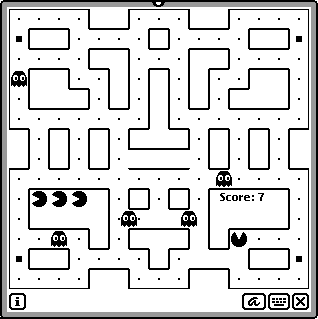
\includegraphics[width=0.6\linewidth]{images/Pac-Man}
		\end{figure}
		\column{.8\textwidth}
		\begin{tikzpicture}
			\node[state, initial] (w) {wander};
			\node[state, right=3cm of w] (c) {chase};
			\node[state, below=of w] (r) {return};
			\node[state, below=of c, right=3.24cm of r]  (f) {flee};
			
			\draw
				(w) edge[bend left=10, above] node{PM spotted} (c)
				(w) edge[bend left=10, above] node{PM power-up} (f)
				(c) edge[bend left=10, below] node{lost PM} (w)
				(c) edge[right] node{PM power-up} (f)
				(f) edge[bend left=10, below] node{PM power-dn} (w)
				(f) edge[below] node{eaten by PM} (r)
				(r) edge[left] node{reach base} (w);
		\end{tikzpicture}
	\end{columns}
\end{frame}

\begin{frame}{Exkurs: PDA im RL}
	Drehkreuz
	\begin{center}
		\begin{figure}
			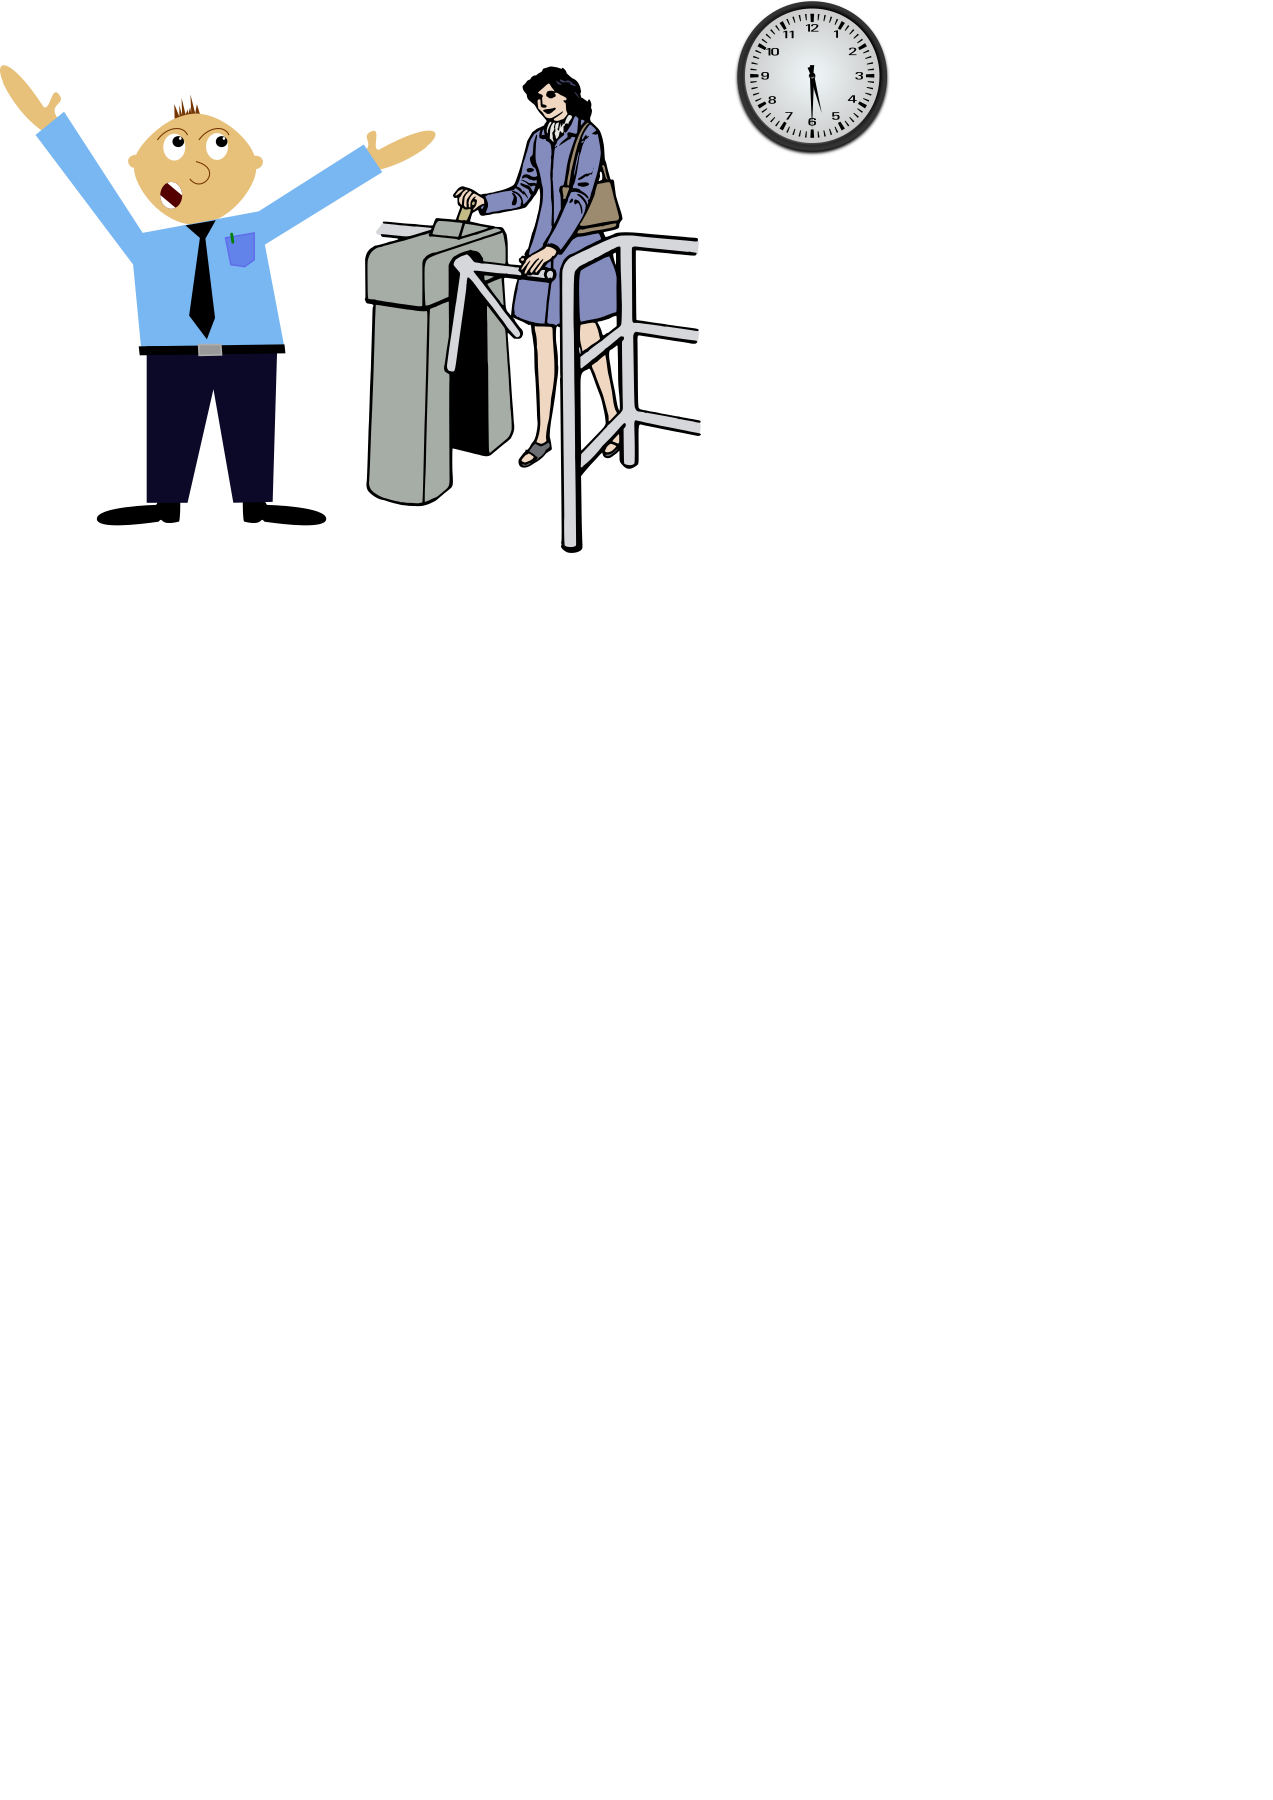
\includegraphics[width=\linewidth]{images/turnstile}
		\end{figure}
	\end{center}
\end{frame}
\section{Kontextfreie Sprachen}

\begin{frame}{Typ-2 Grammatiken: Normalformen}
	\begin{itemize}
		\item Vereinfachungen für kontextfreie Grammatiken $G$
		\begin{itemize}
			\item $G$ reduzieren: nutzlose Variablen eliminieren
			\item Kettenregeln $A \rightarrow B$ entfernen
		\end{itemize}
		\item Chomsky-Normalform
		\begin{itemize}
			\item zu jeder $\varepsilon$-freien, reduzierten kontextfreien Grammatik $G$ ohne Kettenregeln lässt sich eine äquivalente Grammatik $G'$ angeben, die nur Regeln der Art $A \rightarrow a$ bzw. $A \rightarrow BC$ enthält.
			\item Konstuktion: Ausgangspunkt $A\rightarrow X_1X_2 \ldots X_m, m\geq 2, X_i \in V \cup \Sigma$
			\begin{itemize}
				\item für $X_i=a\in \Sigma$ neue Variable $X_a$ mit $X_a \rightarrow a$ einführen
				\item verbleibende Regeln $A \rightarrow B_1B_2\ldots B_m, B_i \in V, m\geq 3$:\\
				ersetze $A \rightarrow B_1D_1, D_1\rightarrow B_2D_2, \ldots, D_{m-2}\rightarrow B_{m-1}B_m$ ($D_i$ neue Variablen)
			\end{itemize}
		\end{itemize}
		\item Greibach-Normalform: Regeln vom Typ $A \rightarrow aB_1B_2 \ldots B_m|a$
	\end{itemize}
\end{frame}

\begin{frame}{Beispiel: Erzeugung Chomsky-Normalform}
	$G=(\{S, A, B\}, \{a, b\}, P, S)$\\
	$P=\{$\\
	\qquad\qquad $S\rightarrow bA|aB$\\
	\qquad\qquad $A\rightarrow bAA|aS|a$\\
	\qquad\qquad $B\rightarrow aBB|bS|b$\\
	\qquad$\}$
\end{frame}

\note{
	\begin{tabular}{rl}
		alt & neu \\
		$S \rightarrow bA$ & $D_b \rightarrow b, S \rightarrow X_bA$ \\
		$S \rightarrow aB$ & $D_a \rightarrow a, S \rightarrow X_aB$ \\
		$A \rightarrow bAA$ & $A \rightarrow X_bAA$ (muss weiter ersetzt werden) \\
		$A \rightarrow aS$ & $A \rightarrow X_aS$ \\
		$B \rightarrow aBB$ & $B \rightarrow X_aBB$ (muss weiter ersetzt werden)\\
		$B \rightarrow bS$ & $B \rightarrow X_bS$ \\
		$A \rightarrow X_bAA$ & $A \rightarrow X_bD_1, D_1 \rightarrow AA$\\
		$B \rightarrow X_aBB$ & $B \rightarrow X_aD_2, D_2 \rightarrow BB$\\
	\end{tabular}
}

\begin{frame}{Worterkennung: CYK-Algorithmus}
	polynomiell auch für nichtdeterministische Sprachen
	\begin{itemize}
		\item Ziel: Worterkennung und Konstruktion Ableitungsbaum bottom-up
		\item Ausgangspunkt: $G$ in Chomsky-Normalform, $w=a_1a_2 \ldots a_n \in \Sigma^*$
		\item definiere $V[i,j]:=\{A \in V \mid A \underset{G}{\Rightarrow}^* w_{ij} \}$ mit\\
		$w_{ij}=a_ia_{i+1}\ldots a_{i+j-1}, |w_{ij}|=j, 1\leq i \leq n, 1\leq j \leq n+1-i$
		\item es gilt: $w\in L$ gdw. $S \in V[1,n]$
		\item schrittweise Berechnug (Rückführung auf kürzere Teilworte)\\
		$j=1: V[i,1]=\{X \in V \mid (X\rightarrow a_i) \in P\}$\\
		$j>1: V[i,j]=\bigcup_{l=1}^{j-1}\{A\in V\mid \exists (A\rightarrow BC): B \in V[i,l] \land C \in V[i+l, j-l] \}$
		\item Wortproblem mit polynomiellem Zeitaufwand $O(n^3)$ lösbar
		\item Grammatik ist mehrdeutig, falls ein $V[i,j]$ mehrere Einträge hat, die von $S$ aus erreicht werden können
	\end{itemize}
\end{frame}

\begin{frame}{Beispiel: CYK-Algorithmus}
	$L=\{a^nb^n\mid n\geq 1\}$\\
	$G=(\{A, B, C, S\}, \{a, b\}, P, S)$\\
	$P=\{S \rightarrow AB|AC, C\rightarrow SB, A\rightarrow a, B\rightarrow b\}$
\end{frame}

\note{
	Betrachten des Wortes $w=aabb$\\
	\begin{columns}
		\column{.5\textwidth}
		\begin{itemize}
			\item[$(a)$] $V[1,1]=\{A\}$
			\item[$(a)$] $V[2,1]=\{A\}$
			\item[$(b)$] $V[3,1]=\{B\}$
			\item[$(b)$] $V[4,1]=\{B\}$
			\item[$(aa)$] $V[1,2]=\varnothing$
		\end{itemize}
		\column{.5\textwidth}
		\begin{itemize}
			\item[$(ab)$] $V[2,2]=\{S\}$
			\item[$(bb)$] $V[3,2]=\varnothing$
			\item[$(aab)$] $V[1,3]=\varnothing$
			\item[$(abb)$] $V[2,3]=\{C\} (l=2)$
			\item[$(aabb)$] $V[1,4]=\{S\} (l=1)$
		\end{itemize}
	\end{columns}
}

\begin{frame}{Pumping-Lemma für kontextfreie Sprachen}
	\begin{itemize}
		\item Pumping-Lemma: für jede kontextfreie Sprache $L$ gilt\\
		es existiert eine natürliche Zahl $n$ so, dass für alle $z \in L$ mit $|z|\geq n$ gilt:\\
		$z$ lässt sich zerlegen in $z=uvwxy$ mit
		\begin{itemize}
			\item $|vx|\geq 1$
			\item $|vwx| \leq n$
			\item $uv^iwx^iy \in L, i=0, 1, 2, \ldots$
		\end{itemize}
		\item Beweis:
		\begin{itemize}
			\item wähle $n=2^m$, $m$: Anzahl der Nichtterminalsymbole, wenn sich G in Chomsky-Normalform befindet
			\item mindestens eine Variable $A$ muss sich im Ableitungsbaum nach spätestens $m$ Schritten wiederholen;\\
			$A\underset{G}{\Rightarrow}^*\omega_1 A \omega_2$, wähle $v: \omega_1 \underset{G}{\Rightarrow}^* v, x: \omega_2 \underset{G}{\Rightarrow}^* x, w: A \underset{G}{\Rightarrow}^* w$;\\
			diese Ableitungen enthalten jeweils keine Wiederholungen von Variablen
		\end{itemize}
	\end{itemize}
\end{frame}

\begin{frame}{Beispiel: Pumping-Lemma für kontextfreie Sprachen}
	$L=\{a^ib^ic^i \mid i\geq 1 \}$
	\begin{itemize}
		\item $L$ ist kontext-sensitiv: Beweis Typ-1-Grammatik\\
		$G=(V, \Sigma, P, S), V=\{S, B, C\}$\\
		$P=\{S\rightarrow aSBC | aBC, CB \rightarrow BC,$\\
		\qquad $aB \rightarrow ab, bB \rightarrow bb, bC \rightarrow bc, cC \rightarrow cc \}$
		\item $L$ ist nicht kontextfrei: Beweis Pumping-Lemma\\
		wäre $L$ kontextfrei, sei $n$ das "`Pumping-$n$"'\\
		wähle $z=a^nb^nc^n \in L, |z|=3n \geq n$\\
		es ex. eine Zerlegung $z=uvwxa$ mit $|vx|\geq 1, |vwx| \leq n$\\
		$\rightarrow$ $vwx$ kann höchstens zwei verschiedene Buchstaben enthalten\\
		$\rightarrow$ in $uv^iwx^iy$ werden ein oder zwei Buchstaben "`aufgepumpt"', der dritte nicht\\
		$\rightarrow$ $uv^iwx^iy \notin L$ für $i \neq 1$ \lightning 
	\end{itemize}
\end{frame}

\begin{frame}{Abschlusseigenschaften kontextfreier Sprachen}
	\begin{itemize}
		\item Kontextfreie Sprachen sind abgeschlossen unter
		\begin{itemize}
			\item Vereinigung: $L_1\cup L_2$\qquad $S \rightarrow S_1|S_2$
			\item Konkatenation: $L_1L_2$ \qquad $S\rightarrow S_1S_2$
			\item Stern-Produkt: $L^*$ \qquad $S_0\rightarrow S|\varepsilon, S\rightarrow S_1|S_1S$
			\item Spiegelung: ersetze in Chomsky-Normalform $A\rightarrow BC$ durch $A \rightarrow BC$
		\end{itemize}
		\item Kontextfreie Sprachen sind \underline{nicht} abgeschlossen unter
		\begin{itemize}
			\item [a)] Durchschnitt\\
			Gegenbeispiel: $L_1=\{a^kb^kc^l\mid k,l\geq 0\}, L_2=\{a^kb^lc^l\mid k,l\geq 0\}$ sind kontextfrei\\
			$L=L_1\cap L_2$ ist nicht kontextfrei
			\item [b)] Komplement\\
			$L_1 \cap L_2 = \overline{\overline{L_1} \cup \overline{L_2}}$: Abgeschlossenheit unter Vereinigung und Komplement würde zu Abgeschlossenheit unter Durchschnitt führen\\
			$\rightarrow$ Widerspruch zu a) \lightning
			
		\end{itemize}
	\end{itemize}
\end{frame}

\begin{frame}{Abschlusseigenschaften deterministisch kontextfreier Sprachen}
	\begin{enumerate}[a)]
		\item Deterministisch kontextfreie Sprachen sind abgeschlossen unter Komplementbildung (beachte: Akzeptanz durch Endzustand!)
		\item Deterministisch kontextfreie Sprachen sind \underline{nicht} abgeschlossen unter
		\begin{enumerate}[i.]
			\item Durchschnitt $L_1 \cap L_2$
			\item Konkatenation $L_1L_2$
			\item Stern-Produkt $L^*$
			\item Vereinigung $L_1 \cup L_2$
		\end{enumerate}
		\item $L_1 \cap L_2$ ist allerdings det. kontextfrei (bzw. kontextfrei) falls $L_1$ regulär und $L_2$ det. kontextfrei (bzw. kontextfrei) ist
	\end{enumerate}
\end{frame}
\section{Typ-0-Sprachen und Turing-Maschinen}

\end{document}

